\documentclass[twoside]{book}

% Packages required by doxygen
\usepackage{fixltx2e}
\usepackage{calc}
\usepackage{doxygen}
\usepackage[export]{adjustbox} % also loads graphicx
\usepackage{graphicx}
\usepackage[utf8]{inputenc}
\usepackage{makeidx}
\usepackage{multicol}
\usepackage{multirow}
\PassOptionsToPackage{warn}{textcomp}
\usepackage{textcomp}
\usepackage[nointegrals]{wasysym}
\usepackage[table]{xcolor}

% NLS support packages
\usepackage[brazil]{babel}
% Font selection
\usepackage[T1]{fontenc}
\usepackage[scaled=.90]{helvet}
\usepackage{courier}
\usepackage{amssymb}
\usepackage{sectsty}
\renewcommand{\familydefault}{\sfdefault}
\allsectionsfont{%
  \fontseries{bc}\selectfont%
  \color{darkgray}%
}
\renewcommand{\DoxyLabelFont}{%
  \fontseries{bc}\selectfont%
  \color{darkgray}%
}
\newcommand{\+}{\discretionary{\mbox{\scriptsize$\hookleftarrow$}}{}{}}

% Page & text layout
\usepackage{geometry}
\geometry{%
  a4paper,%
  top=2.5cm,%
  bottom=2.5cm,%
  left=2.5cm,%
  right=2.5cm%
}
\tolerance=750
\hfuzz=15pt
\hbadness=750
\setlength{\emergencystretch}{15pt}
\setlength{\parindent}{0cm}
\setlength{\parskip}{3ex plus 2ex minus 2ex}
\makeatletter
\renewcommand{\paragraph}{%
  \@startsection{paragraph}{4}{0ex}{-1.0ex}{1.0ex}{%
    \normalfont\normalsize\bfseries\SS@parafont%
  }%
}
\renewcommand{\subparagraph}{%
  \@startsection{subparagraph}{5}{0ex}{-1.0ex}{1.0ex}{%
    \normalfont\normalsize\bfseries\SS@subparafont%
  }%
}
\makeatother

% Headers & footers
\usepackage{fancyhdr}
\pagestyle{fancyplain}
\fancyhead[LE]{\fancyplain{}{\bfseries\thepage}}
\fancyhead[CE]{\fancyplain{}{}}
\fancyhead[RE]{\fancyplain{}{\bfseries\leftmark}}
\fancyhead[LO]{\fancyplain{}{\bfseries\rightmark}}
\fancyhead[CO]{\fancyplain{}{}}
\fancyhead[RO]{\fancyplain{}{\bfseries\thepage}}
\fancyfoot[LE]{\fancyplain{}{}}
\fancyfoot[CE]{\fancyplain{}{}}
\fancyfoot[RE]{\fancyplain{}{\bfseries\scriptsize Gerado por Doxygen }}
\fancyfoot[LO]{\fancyplain{}{\bfseries\scriptsize Gerado por Doxygen }}
\fancyfoot[CO]{\fancyplain{}{}}
\fancyfoot[RO]{\fancyplain{}{}}
\renewcommand{\footrulewidth}{0.4pt}
\renewcommand{\chaptermark}[1]{%
  \markboth{#1}{}%
}
\renewcommand{\sectionmark}[1]{%
  \markright{\thesection\ #1}%
}

% Indices & bibliography
\usepackage{natbib}
\usepackage[titles]{tocloft}
\setcounter{tocdepth}{3}
\setcounter{secnumdepth}{5}
\makeindex

% Hyperlinks (required, but should be loaded last)
\usepackage{ifpdf}
\ifpdf
  \usepackage[pdftex,pagebackref=true]{hyperref}
\else
  \usepackage[ps2pdf,pagebackref=true]{hyperref}
\fi
\hypersetup{%
  colorlinks=true,%
  linkcolor=blue,%
  citecolor=blue,%
  unicode%
}

% Custom commands
\newcommand{\clearemptydoublepage}{%
  \newpage{\pagestyle{empty}\cleardoublepage}%
}

\usepackage{caption}
\captionsetup{labelsep=space,justification=centering,font={bf},singlelinecheck=off,skip=4pt,position=top}

%===== C O N T E N T S =====

\begin{document}

% Titlepage & ToC
\hypersetup{pageanchor=false,
             bookmarksnumbered=true,
             pdfencoding=unicode
            }
\pagenumbering{roman}
\begin{titlepage}
\vspace*{7cm}
\begin{center}%
{\Large Shiba\+Rides }\\
\vspace*{1cm}
{\large Gerado por Doxygen 1.8.11}\\
\end{center}
\end{titlepage}
\clearemptydoublepage
\tableofcontents
\clearemptydoublepage
\pagenumbering{arabic}
\hypersetup{pageanchor=true}

%--- Begin generated contents ---
\chapter{Índice Hierárquico}
\section{Hierarquia de Classes}
Esta lista de hierarquias está parcialmente ordenada (ordem alfabética)\+:\begin{DoxyCompactList}
\item \contentsline{section}{shibarides\+:\+:Carona}{\pageref{classshibarides_1_1Carona}}{}
\item \contentsline{section}{shibarides\+:\+:Conta}{\pageref{classshibarides_1_1Conta}}{}
\item \contentsline{section}{shibarides\+:\+:Dominio}{\pageref{classshibarides_1_1Dominio}}{}
\begin{DoxyCompactList}
\item \contentsline{section}{shibarides\+:\+:Assento}{\pageref{classshibarides_1_1Assento}}{}
\item \contentsline{section}{shibarides\+:\+:Bagagem}{\pageref{classshibarides_1_1Bagagem}}{}
\item \contentsline{section}{shibarides\+:\+:Cidade}{\pageref{classshibarides_1_1Cidade}}{}
\item \contentsline{section}{shibarides\+:\+:Cod\+De\+Banco}{\pageref{classshibarides_1_1CodDeBanco}}{}
\item \contentsline{section}{shibarides\+:\+:Cod\+De\+Carona}{\pageref{classshibarides_1_1CodDeCarona}}{}
\item \contentsline{section}{shibarides\+:\+:Cod\+De\+Reserva}{\pageref{classshibarides_1_1CodDeReserva}}{}
\item \contentsline{section}{shibarides\+:\+:C\+PF}{\pageref{classshibarides_1_1CPF}}{}
\item \contentsline{section}{shibarides\+:\+:Data}{\pageref{classshibarides_1_1Data}}{}
\item \contentsline{section}{shibarides\+:\+:Duracao}{\pageref{classshibarides_1_1Duracao}}{}
\item \contentsline{section}{shibarides\+:\+:Email}{\pageref{classshibarides_1_1Email}}{}
\item \contentsline{section}{shibarides\+:\+:Estado}{\pageref{classshibarides_1_1Estado}}{}
\item \contentsline{section}{shibarides\+:\+:Nome}{\pageref{classshibarides_1_1Nome}}{}
\item \contentsline{section}{shibarides\+:\+:Num\+De\+Agencia}{\pageref{classshibarides_1_1NumDeAgencia}}{}
\item \contentsline{section}{shibarides\+:\+:Num\+De\+Conta}{\pageref{classshibarides_1_1NumDeConta}}{}
\item \contentsline{section}{shibarides\+:\+:Preco}{\pageref{classshibarides_1_1Preco}}{}
\item \contentsline{section}{shibarides\+:\+:Senha}{\pageref{classshibarides_1_1Senha}}{}
\item \contentsline{section}{shibarides\+:\+:Telefone}{\pageref{classshibarides_1_1Telefone}}{}
\item \contentsline{section}{shibarides\+:\+:Vagas}{\pageref{classshibarides_1_1Vagas}}{}
\end{DoxyCompactList}
\item \contentsline{section}{shibarides\+:\+:Reserva}{\pageref{classshibarides_1_1Reserva}}{}
\item \contentsline{section}{shibarides\+:\+:T\+U\+Dominio}{\pageref{classshibarides_1_1TUDominio}}{}
\begin{DoxyCompactList}
\item \contentsline{section}{shibarides\+:\+:T\+U\+Assento}{\pageref{classshibarides_1_1TUAssento}}{}
\item \contentsline{section}{shibarides\+:\+:T\+U\+Bagagem}{\pageref{classshibarides_1_1TUBagagem}}{}
\item \contentsline{section}{shibarides\+:\+:T\+U\+Cidade}{\pageref{classshibarides_1_1TUCidade}}{}
\item \contentsline{section}{shibarides\+:\+:T\+U\+Cod\+De\+Banco}{\pageref{classshibarides_1_1TUCodDeBanco}}{}
\item \contentsline{section}{shibarides\+:\+:T\+U\+Cod\+De\+Carona}{\pageref{classshibarides_1_1TUCodDeCarona}}{}
\item \contentsline{section}{shibarides\+:\+:T\+U\+Cod\+De\+Reserva}{\pageref{classshibarides_1_1TUCodDeReserva}}{}
\item \contentsline{section}{shibarides\+:\+:T\+U\+C\+PF}{\pageref{classshibarides_1_1TUCPF}}{}
\item \contentsline{section}{shibarides\+:\+:T\+U\+Data}{\pageref{classshibarides_1_1TUData}}{}
\item \contentsline{section}{shibarides\+:\+:T\+U\+Duracao}{\pageref{classshibarides_1_1TUDuracao}}{}
\item \contentsline{section}{shibarides\+:\+:T\+U\+Email}{\pageref{classshibarides_1_1TUEmail}}{}
\item \contentsline{section}{shibarides\+:\+:T\+U\+Estado}{\pageref{classshibarides_1_1TUEstado}}{}
\item \contentsline{section}{shibarides\+:\+:T\+U\+Nome}{\pageref{classshibarides_1_1TUNome}}{}
\item \contentsline{section}{shibarides\+:\+:T\+U\+Num\+De\+Agencia}{\pageref{classshibarides_1_1TUNumDeAgencia}}{}
\item \contentsline{section}{shibarides\+:\+:T\+U\+Num\+De\+Conta}{\pageref{classshibarides_1_1TUNumDeConta}}{}
\item \contentsline{section}{shibarides\+:\+:T\+U\+Preco}{\pageref{classshibarides_1_1TUPreco}}{}
\item \contentsline{section}{shibarides\+:\+:T\+U\+Senha}{\pageref{classshibarides_1_1TUSenha}}{}
\item \contentsline{section}{shibarides\+:\+:T\+U\+Telefone}{\pageref{classshibarides_1_1TUTelefone}}{}
\item \contentsline{section}{shibarides\+:\+:T\+U\+Vagas}{\pageref{classshibarides_1_1TUVagas}}{}
\end{DoxyCompactList}
\item \contentsline{section}{shibarides\+:\+:T\+U\+Entidade}{\pageref{classshibarides_1_1TUEntidade}}{}
\begin{DoxyCompactList}
\item \contentsline{section}{shibarides\+:\+:T\+U\+Carona}{\pageref{classshibarides_1_1TUCarona}}{}
\item \contentsline{section}{shibarides\+:\+:T\+U\+Conta}{\pageref{classshibarides_1_1TUConta}}{}
\item \contentsline{section}{shibarides\+:\+:T\+U\+Reserva}{\pageref{classshibarides_1_1TUReserva}}{}
\item \contentsline{section}{shibarides\+:\+:T\+U\+Usuario}{\pageref{classshibarides_1_1TUUsuario}}{}
\end{DoxyCompactList}
\item \contentsline{section}{shibarides\+:\+:Usuario}{\pageref{classshibarides_1_1Usuario}}{}
\end{DoxyCompactList}

\chapter{Índice dos Componentes}
\section{Lista de Componentes}
Aqui estão as classes, estruturas, uniões e interfaces e suas respectivas descrições\+:\begin{DoxyCompactList}
\item\contentsline{section}{\hyperlink{classshibarides_1_1Assento}{shibarides\+::\+Assento} \\*\hyperlink{classshibarides_1_1Dominio}{Dominio} responsável pela preferência de assento do passageiro }{\pageref{classshibarides_1_1Assento}}{}
\item\contentsline{section}{\hyperlink{classshibarides_1_1Bagagem}{shibarides\+::\+Bagagem} \\*\hyperlink{classshibarides_1_1Dominio}{Dominio} responsável pelo numero de volumes da bagagem do passageiro }{\pageref{classshibarides_1_1Bagagem}}{}
\item\contentsline{section}{\hyperlink{classshibarides_1_1Carona}{shibarides\+::\+Carona} }{\pageref{classshibarides_1_1Carona}}{}
\item\contentsline{section}{\hyperlink{classshibarides_1_1Cidade}{shibarides\+::\+Cidade} \\*\hyperlink{classshibarides_1_1Dominio}{Dominio} responsável pelas cidades de origem e destino das caronas }{\pageref{classshibarides_1_1Cidade}}{}
\item\contentsline{section}{\hyperlink{classshibarides_1_1CodDeBanco}{shibarides\+::\+Cod\+De\+Banco} \\*\hyperlink{classshibarides_1_1Dominio}{Dominio} responsável pelo código de banco, fornecido pelo usuaŕio }{\pageref{classshibarides_1_1CodDeBanco}}{}
\item\contentsline{section}{\hyperlink{classshibarides_1_1CodDeCarona}{shibarides\+::\+Cod\+De\+Carona} \\*\hyperlink{classshibarides_1_1Dominio}{Dominio} responsável pelo código da carona fornecida pelo usuaŕio }{\pageref{classshibarides_1_1CodDeCarona}}{}
\item\contentsline{section}{\hyperlink{classshibarides_1_1CodDeReserva}{shibarides\+::\+Cod\+De\+Reserva} \\*\hyperlink{classshibarides_1_1Dominio}{Dominio} responsável pelo código de reserva, fornecido pelo sistema }{\pageref{classshibarides_1_1CodDeReserva}}{}
\item\contentsline{section}{\hyperlink{classshibarides_1_1Conta}{shibarides\+::\+Conta} }{\pageref{classshibarides_1_1Conta}}{}
\item\contentsline{section}{\hyperlink{classshibarides_1_1CPF}{shibarides\+::\+C\+PF} \\*\hyperlink{classshibarides_1_1Dominio}{Dominio} responsável pela validação do \hyperlink{classshibarides_1_1CPF}{C\+PF} }{\pageref{classshibarides_1_1CPF}}{}
\item\contentsline{section}{\hyperlink{classshibarides_1_1Data}{shibarides\+::\+Data} \\*\hyperlink{classshibarides_1_1Dominio}{Dominio} responsável pelas datas }{\pageref{classshibarides_1_1Data}}{}
\item\contentsline{section}{\hyperlink{classshibarides_1_1Dominio}{shibarides\+::\+Dominio} \\*Classe abstrata que serve de base para os domínios }{\pageref{classshibarides_1_1Dominio}}{}
\item\contentsline{section}{\hyperlink{classshibarides_1_1Duracao}{shibarides\+::\+Duracao} \\*\hyperlink{classshibarides_1_1Dominio}{Dominio} responsável pela duração das viagens }{\pageref{classshibarides_1_1Duracao}}{}
\item\contentsline{section}{\hyperlink{classshibarides_1_1Email}{shibarides\+::\+Email} \\*\hyperlink{classshibarides_1_1Dominio}{Dominio} responsável pela validação dos endereços de \hyperlink{classshibarides_1_1Email}{Email} }{\pageref{classshibarides_1_1Email}}{}
\item\contentsline{section}{\hyperlink{classshibarides_1_1Estado}{shibarides\+::\+Estado} \\*\hyperlink{classshibarides_1_1Dominio}{Dominio} responsável pelos estados de origem e destino das viagens }{\pageref{classshibarides_1_1Estado}}{}
\item\contentsline{section}{\hyperlink{classshibarides_1_1Nome}{shibarides\+::\+Nome} }{\pageref{classshibarides_1_1Nome}}{}
\item\contentsline{section}{\hyperlink{classshibarides_1_1NumDeAgencia}{shibarides\+::\+Num\+De\+Agencia} }{\pageref{classshibarides_1_1NumDeAgencia}}{}
\item\contentsline{section}{\hyperlink{classshibarides_1_1NumDeConta}{shibarides\+::\+Num\+De\+Conta} }{\pageref{classshibarides_1_1NumDeConta}}{}
\item\contentsline{section}{\hyperlink{classshibarides_1_1Preco}{shibarides\+::\+Preco} }{\pageref{classshibarides_1_1Preco}}{}
\item\contentsline{section}{\hyperlink{classshibarides_1_1Reserva}{shibarides\+::\+Reserva} }{\pageref{classshibarides_1_1Reserva}}{}
\item\contentsline{section}{\hyperlink{classshibarides_1_1Senha}{shibarides\+::\+Senha} }{\pageref{classshibarides_1_1Senha}}{}
\item\contentsline{section}{\hyperlink{classshibarides_1_1Telefone}{shibarides\+::\+Telefone} }{\pageref{classshibarides_1_1Telefone}}{}
\item\contentsline{section}{\hyperlink{classshibarides_1_1TUAssento}{shibarides\+::\+T\+U\+Assento} }{\pageref{classshibarides_1_1TUAssento}}{}
\item\contentsline{section}{\hyperlink{classshibarides_1_1TUBagagem}{shibarides\+::\+T\+U\+Bagagem} }{\pageref{classshibarides_1_1TUBagagem}}{}
\item\contentsline{section}{\hyperlink{classshibarides_1_1TUCidade}{shibarides\+::\+T\+U\+Cidade} }{\pageref{classshibarides_1_1TUCidade}}{}
\item\contentsline{section}{\hyperlink{classshibarides_1_1TUCodDeBanco}{shibarides\+::\+T\+U\+Cod\+De\+Banco} }{\pageref{classshibarides_1_1TUCodDeBanco}}{}
\item\contentsline{section}{\hyperlink{classshibarides_1_1TUCodDeCarona}{shibarides\+::\+T\+U\+Cod\+De\+Carona} }{\pageref{classshibarides_1_1TUCodDeCarona}}{}
\item\contentsline{section}{\hyperlink{classshibarides_1_1TUCodDeReserva}{shibarides\+::\+T\+U\+Cod\+De\+Reserva} }{\pageref{classshibarides_1_1TUCodDeReserva}}{}
\item\contentsline{section}{\hyperlink{classshibarides_1_1TUConta}{shibarides\+::\+T\+U\+Conta} }{\pageref{classshibarides_1_1TUConta}}{}
\item\contentsline{section}{\hyperlink{classshibarides_1_1TUCPF}{shibarides\+::\+T\+U\+C\+PF} }{\pageref{classshibarides_1_1TUCPF}}{}
\item\contentsline{section}{\hyperlink{classshibarides_1_1TUData}{shibarides\+::\+T\+U\+Data} }{\pageref{classshibarides_1_1TUData}}{}
\item\contentsline{section}{\hyperlink{classshibarides_1_1TUDominio}{shibarides\+::\+T\+U\+Dominio} }{\pageref{classshibarides_1_1TUDominio}}{}
\item\contentsline{section}{\hyperlink{classshibarides_1_1TUDuracao}{shibarides\+::\+T\+U\+Duracao} }{\pageref{classshibarides_1_1TUDuracao}}{}
\item\contentsline{section}{\hyperlink{classshibarides_1_1TUEmail}{shibarides\+::\+T\+U\+Email} }{\pageref{classshibarides_1_1TUEmail}}{}
\item\contentsline{section}{\hyperlink{classshibarides_1_1TUEntidade}{shibarides\+::\+T\+U\+Entidade} }{\pageref{classshibarides_1_1TUEntidade}}{}
\item\contentsline{section}{\hyperlink{classshibarides_1_1TUEstado}{shibarides\+::\+T\+U\+Estado} }{\pageref{classshibarides_1_1TUEstado}}{}
\item\contentsline{section}{\hyperlink{classshibarides_1_1TUNome}{shibarides\+::\+T\+U\+Nome} }{\pageref{classshibarides_1_1TUNome}}{}
\item\contentsline{section}{\hyperlink{classshibarides_1_1TUNumDeAgencia}{shibarides\+::\+T\+U\+Num\+De\+Agencia} }{\pageref{classshibarides_1_1TUNumDeAgencia}}{}
\item\contentsline{section}{\hyperlink{classshibarides_1_1TUNumDeConta}{shibarides\+::\+T\+U\+Num\+De\+Conta} }{\pageref{classshibarides_1_1TUNumDeConta}}{}
\item\contentsline{section}{\hyperlink{classshibarides_1_1TUPreco}{shibarides\+::\+T\+U\+Preco} }{\pageref{classshibarides_1_1TUPreco}}{}
\item\contentsline{section}{\hyperlink{classshibarides_1_1TUReserva}{shibarides\+::\+T\+U\+Reserva} }{\pageref{classshibarides_1_1TUReserva}}{}
\item\contentsline{section}{\hyperlink{classshibarides_1_1TUSenha}{shibarides\+::\+T\+U\+Senha} }{\pageref{classshibarides_1_1TUSenha}}{}
\item\contentsline{section}{\hyperlink{classshibarides_1_1TUTelefone}{shibarides\+::\+T\+U\+Telefone} }{\pageref{classshibarides_1_1TUTelefone}}{}
\item\contentsline{section}{\hyperlink{classshibarides_1_1TUUsuario}{shibarides\+::\+T\+U\+Usuario} }{\pageref{classshibarides_1_1TUUsuario}}{}
\item\contentsline{section}{\hyperlink{classshibarides_1_1TUVagas}{shibarides\+::\+T\+U\+Vagas} }{\pageref{classshibarides_1_1TUVagas}}{}
\item\contentsline{section}{\hyperlink{classshibarides_1_1Usuario}{shibarides\+::\+Usuario} }{\pageref{classshibarides_1_1Usuario}}{}
\item\contentsline{section}{\hyperlink{classshibarides_1_1Vagas}{shibarides\+::\+Vagas} }{\pageref{classshibarides_1_1Vagas}}{}
\end{DoxyCompactList}

\chapter{Classes}
\hypertarget{classshibarides_1_1Assento}{}\section{Referência da Classe shibarides\+:\+:Assento}
\label{classshibarides_1_1Assento}\index{shibarides\+::\+Assento@{shibarides\+::\+Assento}}


Diagrama de Hierarquia para shibarides\+:\+:Assento\+:\nopagebreak
\begin{figure}[H]
\begin{center}
\leavevmode
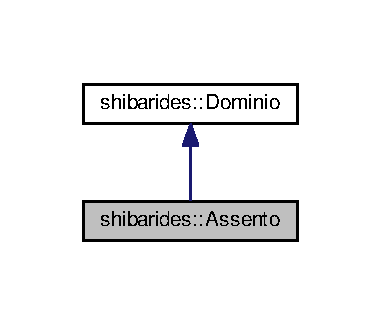
\includegraphics[width=183pt]{classshibarides_1_1Assento__inherit__graph}
\end{center}
\end{figure}


Diagrama de colaboração para shibarides\+:\+:Assento\+:\nopagebreak
\begin{figure}[H]
\begin{center}
\leavevmode
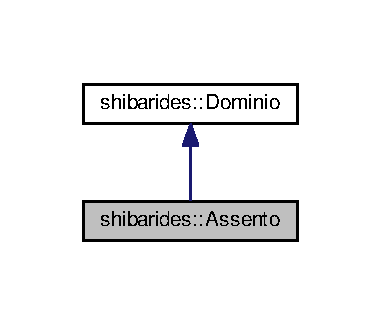
\includegraphics[width=183pt]{classshibarides_1_1Assento__coll__graph}
\end{center}
\end{figure}
\subsection*{Métodos Privados}
\begin{DoxyCompactItemize}
\item 
void \hyperlink{classshibarides_1_1Assento_a8a2099562808c49caff59569bcb977c3}{validate} (std\+::string)  throw (std\+::invalid\+\_\+argument)
\begin{DoxyCompactList}\small\item\em Função privada que define as regras de validação para o dominio. \end{DoxyCompactList}\end{DoxyCompactItemize}
\subsection*{Outros membros herdados}


\subsection{Métodos}
\index{shibarides\+::\+Assento@{shibarides\+::\+Assento}!validate@{validate}}
\index{validate@{validate}!shibarides\+::\+Assento@{shibarides\+::\+Assento}}
\subsubsection[{\texorpdfstring{validate(std\+::string)}{validate(std::string)}}]{\setlength{\rightskip}{0pt plus 5cm}void Assento\+::validate (
\begin{DoxyParamCaption}
\item[{std\+::string}]{}
\end{DoxyParamCaption}
) throw  std\+::invalid\+\_\+argument) \hspace{0.3cm}{\ttfamily [private]}, {\ttfamily [virtual]}}\hypertarget{classshibarides_1_1Assento_a8a2099562808c49caff59569bcb977c3}{}\label{classshibarides_1_1Assento_a8a2099562808c49caff59569bcb977c3}


Função privada que define as regras de validação para o dominio. 

Função pura abstrata, que é sobrescrita nos domínios e define o comportamento de cada domínio. Caso o valor passado nao seja valido, é lançada uma excessão std\+::invalid\+\_\+argument.


\begin{DoxyParams}{Parâmetros}
{\em string} & Valor a ser validado. \\
\hline
\end{DoxyParams}


Implementa \hyperlink{classshibarides_1_1Dominio_acc9445531455c072bbf708709aebbe55}{shibarides\+::\+Dominio}.



A documentação para esta classe foi gerada a partir dos seguintes arquivos\+:\begin{DoxyCompactItemize}
\item 
shibarides/Shiba\+Rides\+Domains.\+hpp\item 
shibarides/Shiba\+Rides\+Domains.\+cpp\end{DoxyCompactItemize}

\hypertarget{classshibarides_1_1Bagagem}{}\section{Referência da Classe shibarides\+:\+:Bagagem}
\label{classshibarides_1_1Bagagem}\index{shibarides\+::\+Bagagem@{shibarides\+::\+Bagagem}}


Diagrama de Hierarquia para shibarides\+:\+:Bagagem\+:\nopagebreak
\begin{figure}[H]
\begin{center}
\leavevmode
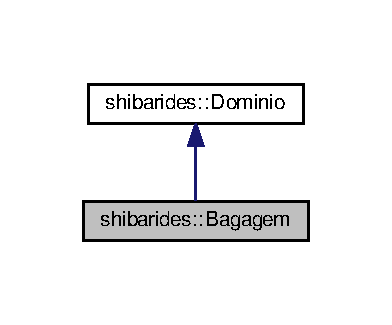
\includegraphics[width=188pt]{classshibarides_1_1Bagagem__inherit__graph}
\end{center}
\end{figure}


Diagrama de colaboração para shibarides\+:\+:Bagagem\+:\nopagebreak
\begin{figure}[H]
\begin{center}
\leavevmode
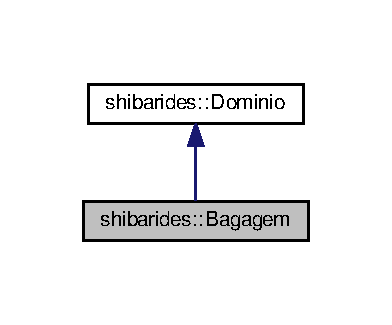
\includegraphics[width=188pt]{classshibarides_1_1Bagagem__coll__graph}
\end{center}
\end{figure}
\subsection*{Métodos Privados}
\begin{DoxyCompactItemize}
\item 
void \hyperlink{classshibarides_1_1Bagagem_aad85c0b035f3f3202130160edc35d41d}{validate} (std\+::string)  throw (std\+::invalid\+\_\+argument)
\begin{DoxyCompactList}\small\item\em Função privada que define as regras de validação para o dominio. \end{DoxyCompactList}\end{DoxyCompactItemize}
\subsection*{Outros membros herdados}


\subsection{Métodos}
\index{shibarides\+::\+Bagagem@{shibarides\+::\+Bagagem}!validate@{validate}}
\index{validate@{validate}!shibarides\+::\+Bagagem@{shibarides\+::\+Bagagem}}
\subsubsection[{\texorpdfstring{validate(std\+::string)}{validate(std::string)}}]{\setlength{\rightskip}{0pt plus 5cm}void Bagagem\+::validate (
\begin{DoxyParamCaption}
\item[{std\+::string}]{}
\end{DoxyParamCaption}
) throw  std\+::invalid\+\_\+argument) \hspace{0.3cm}{\ttfamily [private]}, {\ttfamily [virtual]}}\hypertarget{classshibarides_1_1Bagagem_aad85c0b035f3f3202130160edc35d41d}{}\label{classshibarides_1_1Bagagem_aad85c0b035f3f3202130160edc35d41d}


Função privada que define as regras de validação para o dominio. 

Função pura abstrata, que é sobrescrita nos domínios e define o comportamento de cada domínio. Caso o valor passado nao seja valido, é lançada uma excessão std\+::invalid\+\_\+argument.


\begin{DoxyParams}{Parâmetros}
{\em string} & Valor a ser validado. \\
\hline
\end{DoxyParams}


Implementa \hyperlink{classshibarides_1_1Dominio_acc9445531455c072bbf708709aebbe55}{shibarides\+::\+Dominio}.



A documentação para esta classe foi gerada a partir dos seguintes arquivos\+:\begin{DoxyCompactItemize}
\item 
shibarides/Shiba\+Rides\+Domains.\+hpp\item 
shibarides/Shiba\+Rides\+Domains.\+cpp\end{DoxyCompactItemize}

\hypertarget{classshibarides_1_1Carona}{}\section{Referência da Classe shibarides\+:\+:Carona}
\label{classshibarides_1_1Carona}\index{shibarides\+::\+Carona@{shibarides\+::\+Carona}}


Diagrama de colaboração para shibarides\+:\+:Carona\+:\nopagebreak
\begin{figure}[H]
\begin{center}
\leavevmode
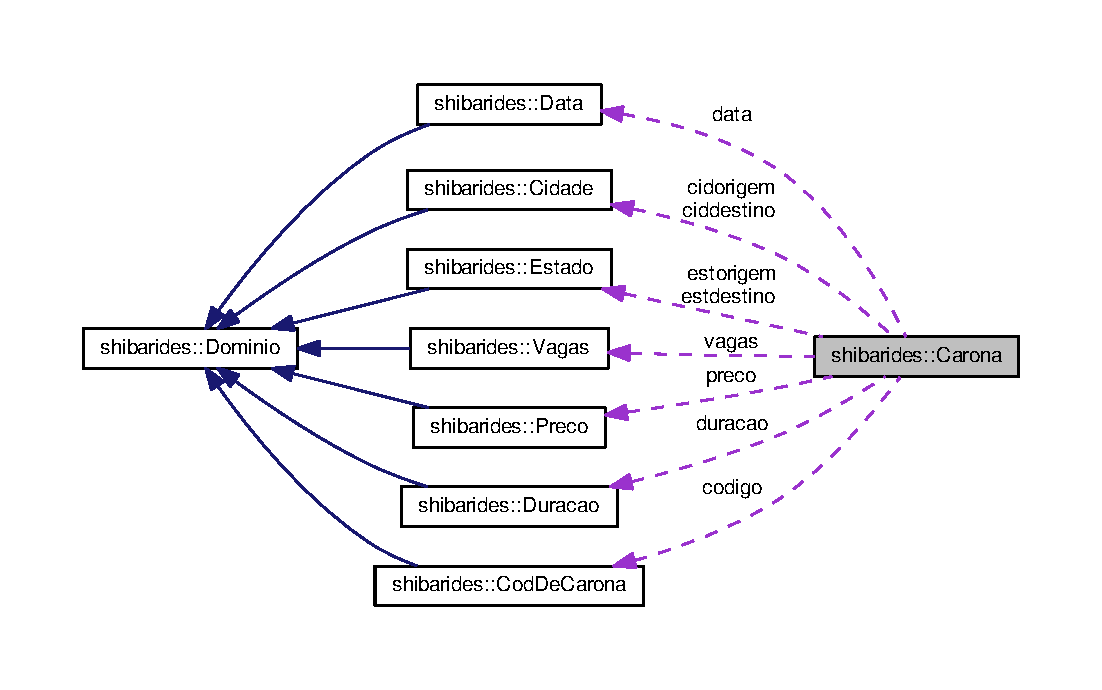
\includegraphics[width=350pt]{classshibarides_1_1Carona__coll__graph}
\end{center}
\end{figure}
\subsection*{Métodos Públicos}
\begin{DoxyCompactItemize}
\item 
void {\bfseries set\+Codigo} (const \hyperlink{classshibarides_1_1CodDeCarona}{Cod\+De\+Carona} \&codigo)\hypertarget{classshibarides_1_1Carona_a4c92ff9279cf52a428b8ff25e6a132db}{}\label{classshibarides_1_1Carona_a4c92ff9279cf52a428b8ff25e6a132db}

\item 
\hyperlink{classshibarides_1_1CodDeCarona}{Cod\+De\+Carona} {\bfseries get\+Codigo} () const \hypertarget{classshibarides_1_1Carona_aaf5471db61f27b78a13798003f12439c}{}\label{classshibarides_1_1Carona_aaf5471db61f27b78a13798003f12439c}

\item 
void {\bfseries set\+Cidade\+Origem} (const \hyperlink{classshibarides_1_1Cidade}{Cidade} \&cidorigem)\hypertarget{classshibarides_1_1Carona_a4a47c7f3210c4e9c2d4c380bd6c66682}{}\label{classshibarides_1_1Carona_a4a47c7f3210c4e9c2d4c380bd6c66682}

\item 
\hyperlink{classshibarides_1_1Cidade}{Cidade} {\bfseries get\+Cidade\+Origem} () const \hypertarget{classshibarides_1_1Carona_a01e2983cc1cf3cb30b550d8a38a7a8e1}{}\label{classshibarides_1_1Carona_a01e2983cc1cf3cb30b550d8a38a7a8e1}

\item 
void {\bfseries set\+Estado\+Origem} (const \hyperlink{classshibarides_1_1Estado}{Estado} \&estorigem)\hypertarget{classshibarides_1_1Carona_a72879cb0fe8fa20c740a3069e835571a}{}\label{classshibarides_1_1Carona_a72879cb0fe8fa20c740a3069e835571a}

\item 
\hyperlink{classshibarides_1_1Estado}{Estado} {\bfseries get\+Estado\+Origem} () const \hypertarget{classshibarides_1_1Carona_a27959baa3fab1df9ebabd62aaa2865a1}{}\label{classshibarides_1_1Carona_a27959baa3fab1df9ebabd62aaa2865a1}

\item 
void {\bfseries set\+Cidade\+Destino} (const \hyperlink{classshibarides_1_1Cidade}{Cidade} \&ciddestino)\hypertarget{classshibarides_1_1Carona_a679af6917e6369980427717f986b139a}{}\label{classshibarides_1_1Carona_a679af6917e6369980427717f986b139a}

\item 
\hyperlink{classshibarides_1_1Cidade}{Cidade} {\bfseries get\+Cidade\+Destino} () const \hypertarget{classshibarides_1_1Carona_a9db3d8d18f6b1395770b93ec79da5406}{}\label{classshibarides_1_1Carona_a9db3d8d18f6b1395770b93ec79da5406}

\item 
void {\bfseries set\+Estado\+Destino} (const \hyperlink{classshibarides_1_1Estado}{Estado} \&estdestino)\hypertarget{classshibarides_1_1Carona_ad45ec8a30c65465ac957c23f2524f2d2}{}\label{classshibarides_1_1Carona_ad45ec8a30c65465ac957c23f2524f2d2}

\item 
\hyperlink{classshibarides_1_1Estado}{Estado} {\bfseries get\+Estado\+Destino} () const \hypertarget{classshibarides_1_1Carona_a6bf4e3a027d39582564fac6691a4ebaa}{}\label{classshibarides_1_1Carona_a6bf4e3a027d39582564fac6691a4ebaa}

\item 
void {\bfseries set\+Data} (const \hyperlink{classshibarides_1_1Data}{Data} \&data)\hypertarget{classshibarides_1_1Carona_a41ec8487483226c682dc23ea0b70dc1f}{}\label{classshibarides_1_1Carona_a41ec8487483226c682dc23ea0b70dc1f}

\item 
\hyperlink{classshibarides_1_1Data}{Data} {\bfseries get\+Data} () const \hypertarget{classshibarides_1_1Carona_a107f7a86aa5208f31982aa19d27643b6}{}\label{classshibarides_1_1Carona_a107f7a86aa5208f31982aa19d27643b6}

\item 
void {\bfseries set\+Duracao} (const \hyperlink{classshibarides_1_1Duracao}{Duracao} \&duracao)\hypertarget{classshibarides_1_1Carona_a3d6564b9ba1e3670d0c8ce87a011b0c3}{}\label{classshibarides_1_1Carona_a3d6564b9ba1e3670d0c8ce87a011b0c3}

\item 
\hyperlink{classshibarides_1_1Duracao}{Duracao} {\bfseries get\+Duracao} () const \hypertarget{classshibarides_1_1Carona_a992c3626a20b5195aca7fb92987c3992}{}\label{classshibarides_1_1Carona_a992c3626a20b5195aca7fb92987c3992}

\item 
void {\bfseries set\+Vagas} (const \hyperlink{classshibarides_1_1Vagas}{Vagas} \&vagas)\hypertarget{classshibarides_1_1Carona_a88df340d8ee646d86e2b5ed20c56dacc}{}\label{classshibarides_1_1Carona_a88df340d8ee646d86e2b5ed20c56dacc}

\item 
\hyperlink{classshibarides_1_1Vagas}{Vagas} {\bfseries get\+Vagas} () const \hypertarget{classshibarides_1_1Carona_abcc251acf0ef08c20b845832d5cba6db}{}\label{classshibarides_1_1Carona_abcc251acf0ef08c20b845832d5cba6db}

\item 
void {\bfseries set\+Preco} (const \hyperlink{classshibarides_1_1Preco}{Preco} \&preco)\hypertarget{classshibarides_1_1Carona_a6db9b66a554694539c5f5aa4f13657a1}{}\label{classshibarides_1_1Carona_a6db9b66a554694539c5f5aa4f13657a1}

\item 
\hyperlink{classshibarides_1_1Preco}{Preco} {\bfseries get\+Preco} () const \hypertarget{classshibarides_1_1Carona_a8ec9d24a04fe95497976b985ec7c6c04}{}\label{classshibarides_1_1Carona_a8ec9d24a04fe95497976b985ec7c6c04}

\end{DoxyCompactItemize}
\subsection*{Atributos Privados}
\begin{DoxyCompactItemize}
\item 
\hyperlink{classshibarides_1_1CodDeCarona}{Cod\+De\+Carona} {\bfseries codigo}\hypertarget{classshibarides_1_1Carona_a7b00981c5d5cea183feb2ca4d760911e}{}\label{classshibarides_1_1Carona_a7b00981c5d5cea183feb2ca4d760911e}

\item 
\hyperlink{classshibarides_1_1Cidade}{Cidade} {\bfseries cidorigem}\hypertarget{classshibarides_1_1Carona_adc888314cb15f45314f7a11e0b05f6d8}{}\label{classshibarides_1_1Carona_adc888314cb15f45314f7a11e0b05f6d8}

\item 
\hyperlink{classshibarides_1_1Estado}{Estado} {\bfseries estorigem}\hypertarget{classshibarides_1_1Carona_a6dace71d7fb30f46f0a16cfd67d26287}{}\label{classshibarides_1_1Carona_a6dace71d7fb30f46f0a16cfd67d26287}

\item 
\hyperlink{classshibarides_1_1Cidade}{Cidade} {\bfseries ciddestino}\hypertarget{classshibarides_1_1Carona_abac6f586588317b57d7c5b83ae3f4c6e}{}\label{classshibarides_1_1Carona_abac6f586588317b57d7c5b83ae3f4c6e}

\item 
\hyperlink{classshibarides_1_1Estado}{Estado} {\bfseries estdestino}\hypertarget{classshibarides_1_1Carona_afc2464789b24fb27ac8b4c769683c90b}{}\label{classshibarides_1_1Carona_afc2464789b24fb27ac8b4c769683c90b}

\item 
\hyperlink{classshibarides_1_1Data}{Data} {\bfseries data}\hypertarget{classshibarides_1_1Carona_abdc97cb7684302dc4d1e580613acd3cc}{}\label{classshibarides_1_1Carona_abdc97cb7684302dc4d1e580613acd3cc}

\item 
\hyperlink{classshibarides_1_1Duracao}{Duracao} {\bfseries duracao}\hypertarget{classshibarides_1_1Carona_aa4434820ca3b9bd4e6b3bfb7d9b6749d}{}\label{classshibarides_1_1Carona_aa4434820ca3b9bd4e6b3bfb7d9b6749d}

\item 
\hyperlink{classshibarides_1_1Vagas}{Vagas} {\bfseries vagas}\hypertarget{classshibarides_1_1Carona_a1bb8450bb0575d860527746cd079f80f}{}\label{classshibarides_1_1Carona_a1bb8450bb0575d860527746cd079f80f}

\item 
\hyperlink{classshibarides_1_1Preco}{Preco} {\bfseries preco}\hypertarget{classshibarides_1_1Carona_a72dbfd71e7f0a54a58f2ff851ead0fc2}{}\label{classshibarides_1_1Carona_a72dbfd71e7f0a54a58f2ff851ead0fc2}

\end{DoxyCompactItemize}


A documentação para esta classe foi gerada a partir do seguinte arquivo\+:\begin{DoxyCompactItemize}
\item 
shibarides/Shiba\+Rides\+Entities.\+hpp\end{DoxyCompactItemize}

\hypertarget{classshibarides_1_1Cidade}{}\section{Referência da Classe shibarides\+:\+:Cidade}
\label{classshibarides_1_1Cidade}\index{shibarides\+::\+Cidade@{shibarides\+::\+Cidade}}


Diagrama de Hierarquia para shibarides\+:\+:Cidade\+:\nopagebreak
\begin{figure}[H]
\begin{center}
\leavevmode
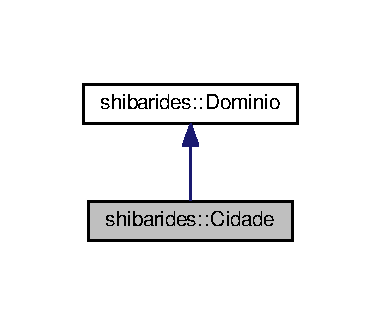
\includegraphics[width=183pt]{classshibarides_1_1Cidade__inherit__graph}
\end{center}
\end{figure}


Diagrama de colaboração para shibarides\+:\+:Cidade\+:\nopagebreak
\begin{figure}[H]
\begin{center}
\leavevmode
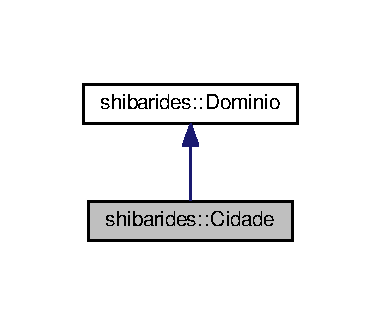
\includegraphics[width=183pt]{classshibarides_1_1Cidade__coll__graph}
\end{center}
\end{figure}
\subsection*{Outros membros herdados}


A documentação para esta classe foi gerada a partir dos seguintes arquivos\+:\begin{DoxyCompactItemize}
\item 
shibarides/Shiba\+Rides\+Domains.\+hpp\item 
shibarides/Shiba\+Rides\+Domains.\+cpp\end{DoxyCompactItemize}

\hypertarget{classshibarides_1_1CodDeBanco}{}\section{Referência da Classe shibarides\+:\+:Cod\+De\+Banco}
\label{classshibarides_1_1CodDeBanco}\index{shibarides\+::\+Cod\+De\+Banco@{shibarides\+::\+Cod\+De\+Banco}}


Diagrama de Hierarquia para shibarides\+:\+:Cod\+De\+Banco\+:
% FIG 0


Diagrama de colaboração para shibarides\+:\+:Cod\+De\+Banco\+:
% FIG 1
\subsection*{Outros membros herdados}


A documentação para esta classe foi gerada a partir dos seguintes arquivos\+:\begin{DoxyCompactItemize}
\item 
shibarides/Shiba\+Rides\+Domains.\+hpp\item 
shibarides/Shiba\+Rides\+Domains.\+cpp\end{DoxyCompactItemize}

\hypertarget{classshibarides_1_1CodDeCarona}{}\section{Referência da Classe shibarides\+:\+:Cod\+De\+Carona}
\label{classshibarides_1_1CodDeCarona}\index{shibarides\+::\+Cod\+De\+Carona@{shibarides\+::\+Cod\+De\+Carona}}


Diagrama de Hierarquia para shibarides\+:\+:Cod\+De\+Carona\+:\nopagebreak
\begin{figure}[H]
\begin{center}
\leavevmode
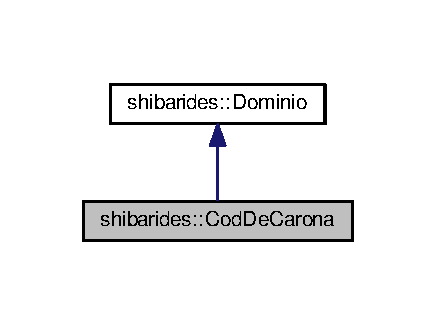
\includegraphics[width=209pt]{classshibarides_1_1CodDeCarona__inherit__graph}
\end{center}
\end{figure}


Diagrama de colaboração para shibarides\+:\+:Cod\+De\+Carona\+:\nopagebreak
\begin{figure}[H]
\begin{center}
\leavevmode
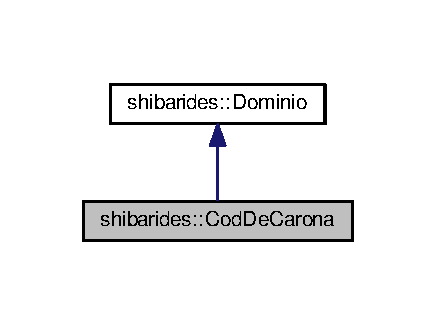
\includegraphics[width=209pt]{classshibarides_1_1CodDeCarona__coll__graph}
\end{center}
\end{figure}
\subsection*{Métodos Privados}
\begin{DoxyCompactItemize}
\item 
void \hyperlink{classshibarides_1_1CodDeCarona_a2713cdc938576b30a6f7e59ddc67a848}{validate} (std\+::string)  throw (std\+::invalid\+\_\+argument)
\begin{DoxyCompactList}\small\item\em Função privada que define as regras de validação para o dominio. \end{DoxyCompactList}\end{DoxyCompactItemize}
\subsection*{Outros membros herdados}


\subsection{Métodos}
\index{shibarides\+::\+Cod\+De\+Carona@{shibarides\+::\+Cod\+De\+Carona}!validate@{validate}}
\index{validate@{validate}!shibarides\+::\+Cod\+De\+Carona@{shibarides\+::\+Cod\+De\+Carona}}
\subsubsection[{\texorpdfstring{validate(std\+::string)}{validate(std::string)}}]{\setlength{\rightskip}{0pt plus 5cm}void Cod\+De\+Carona\+::validate (
\begin{DoxyParamCaption}
\item[{std\+::string}]{}
\end{DoxyParamCaption}
) throw  std\+::invalid\+\_\+argument) \hspace{0.3cm}{\ttfamily [private]}, {\ttfamily [virtual]}}\hypertarget{classshibarides_1_1CodDeCarona_a2713cdc938576b30a6f7e59ddc67a848}{}\label{classshibarides_1_1CodDeCarona_a2713cdc938576b30a6f7e59ddc67a848}


Função privada que define as regras de validação para o dominio. 

Função pura abstrata, que é sobrescrita nos domínios e define o comportamento de cada domínio. Caso o valor passado nao seja valido, é lançada uma excessão std\+::invalid\+\_\+argument.


\begin{DoxyParams}{Parâmetros}
{\em string} & Valor a ser validado. \\
\hline
\end{DoxyParams}


Implementa \hyperlink{classshibarides_1_1Dominio_acc9445531455c072bbf708709aebbe55}{shibarides\+::\+Dominio}.



A documentação para esta classe foi gerada a partir dos seguintes arquivos\+:\begin{DoxyCompactItemize}
\item 
shibarides/Shiba\+Rides\+Domains.\+hpp\item 
shibarides/Shiba\+Rides\+Domains.\+cpp\end{DoxyCompactItemize}

\hypertarget{classshibarides_1_1CodDeReserva}{}\section{Referência da Classe shibarides\+:\+:Cod\+De\+Reserva}
\label{classshibarides_1_1CodDeReserva}\index{shibarides\+::\+Cod\+De\+Reserva@{shibarides\+::\+Cod\+De\+Reserva}}


\hyperlink{classshibarides_1_1Dominio}{Dominio} responsável pelo código de reserva, fornecido pelo sistema.  




{\ttfamily \#include $<$Shiba\+Rides\+Domains.\+hpp$>$}



Diagrama de Hierarquia para shibarides\+:\+:Cod\+De\+Reserva\+:\nopagebreak
\begin{figure}[H]
\begin{center}
\leavevmode
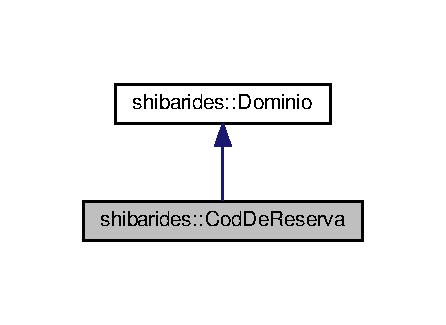
\includegraphics[width=214pt]{classshibarides_1_1CodDeReserva__inherit__graph}
\end{center}
\end{figure}


Diagrama de colaboração para shibarides\+:\+:Cod\+De\+Reserva\+:\nopagebreak
\begin{figure}[H]
\begin{center}
\leavevmode
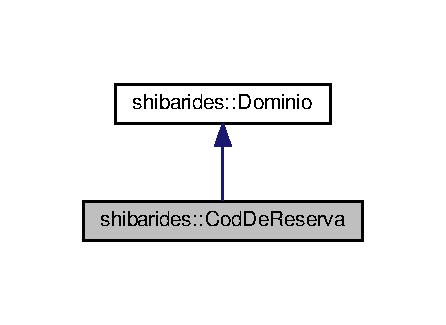
\includegraphics[width=214pt]{classshibarides_1_1CodDeReserva__coll__graph}
\end{center}
\end{figure}
\subsection*{Métodos Privados}
\begin{DoxyCompactItemize}
\item 
void \hyperlink{classshibarides_1_1CodDeReserva_a595a667ca295b1adc5eedefd773d8027}{validate} (std\+::string)  throw (std\+::invalid\+\_\+argument)
\begin{DoxyCompactList}\small\item\em Método que define as regras de validação para o dominio. \end{DoxyCompactList}\end{DoxyCompactItemize}
\subsection*{Outros membros herdados}


\subsection{Descrição Detalhada}
\hyperlink{classshibarides_1_1Dominio}{Dominio} responsável pelo código de reserva, fornecido pelo sistema. 

Representa o código de reserva feita pelo usuario. Os valores aceitos são da forma X\+X\+X\+XX, onde X é dígito de 0 a 9. 

\subsection{Métodos}
\index{shibarides\+::\+Cod\+De\+Reserva@{shibarides\+::\+Cod\+De\+Reserva}!validate@{validate}}
\index{validate@{validate}!shibarides\+::\+Cod\+De\+Reserva@{shibarides\+::\+Cod\+De\+Reserva}}
\subsubsection[{\texorpdfstring{validate(std\+::string)}{validate(std::string)}}]{\setlength{\rightskip}{0pt plus 5cm}void Cod\+De\+Reserva\+::validate (
\begin{DoxyParamCaption}
\item[{std\+::string}]{value}
\end{DoxyParamCaption}
) throw  std\+::invalid\+\_\+argument) \hspace{0.3cm}{\ttfamily [private]}, {\ttfamily [virtual]}}\hypertarget{classshibarides_1_1CodDeReserva_a595a667ca295b1adc5eedefd773d8027}{}\label{classshibarides_1_1CodDeReserva_a595a667ca295b1adc5eedefd773d8027}


Método que define as regras de validação para o dominio. 

O método validate implementa as regras de validação para o dominio. Os valores aceitos para este dominio são da forma X\+X\+X\+XX, onde X é dígito de 0 a 9.


\begin{DoxyParams}{Parâmetros}
{\em value} & Valor a ser validado \\
\hline
\end{DoxyParams}


Implementa \hyperlink{classshibarides_1_1Dominio_acc9445531455c072bbf708709aebbe55}{shibarides\+::\+Dominio}.



A documentação para esta classe foi gerada a partir dos seguintes arquivos\+:\begin{DoxyCompactItemize}
\item 
shibarides/domains/Shiba\+Rides\+Domains.\+hpp\item 
shibarides/domains/Shiba\+Rides\+Domains.\+cpp\end{DoxyCompactItemize}

\hypertarget{classshibarides_1_1Conta}{}\section{Referência da Classe shibarides\+:\+:Conta}
\label{classshibarides_1_1Conta}\index{shibarides\+::\+Conta@{shibarides\+::\+Conta}}
\subsection*{Métodos Públicos}
\begin{DoxyCompactItemize}
\item 
void {\bfseries set\+Banco} (const \hyperlink{classshibarides_1_1CodDeBanco}{Cod\+De\+Banco} \&banco)\hypertarget{classshibarides_1_1Conta_a9300f2180e88b9df87343193c926badf}{}\label{classshibarides_1_1Conta_a9300f2180e88b9df87343193c926badf}

\item 
\hyperlink{classshibarides_1_1CodDeBanco}{Cod\+De\+Banco} {\bfseries get\+Banco} () const \hypertarget{classshibarides_1_1Conta_a40bb0d5f152f61b26a7bd6174af1124f}{}\label{classshibarides_1_1Conta_a40bb0d5f152f61b26a7bd6174af1124f}

\item 
void {\bfseries set\+Agencia} (const \hyperlink{classshibarides_1_1NumDeAgencia}{Num\+De\+Agencia} \&agencia)\hypertarget{classshibarides_1_1Conta_a53957be04cf0cd5a7fb783c7d320aa74}{}\label{classshibarides_1_1Conta_a53957be04cf0cd5a7fb783c7d320aa74}

\item 
\hyperlink{classshibarides_1_1NumDeAgencia}{Num\+De\+Agencia} {\bfseries get\+Agencia} () const \hypertarget{classshibarides_1_1Conta_a4131ed3a711e4dd69a9adf3f66cb9abc}{}\label{classshibarides_1_1Conta_a4131ed3a711e4dd69a9adf3f66cb9abc}

\item 
void {\bfseries set\+Conta} (const \hyperlink{classshibarides_1_1NumDeConta}{Num\+De\+Conta} \&conta)\hypertarget{classshibarides_1_1Conta_ac04fa978221a3b76cd64878ad6853dc7}{}\label{classshibarides_1_1Conta_ac04fa978221a3b76cd64878ad6853dc7}

\item 
\hyperlink{classshibarides_1_1NumDeConta}{Num\+De\+Conta} {\bfseries get\+Conta} () const \hypertarget{classshibarides_1_1Conta_a0f18603982a99ab28e89207ed6bbe96c}{}\label{classshibarides_1_1Conta_a0f18603982a99ab28e89207ed6bbe96c}

\end{DoxyCompactItemize}


A documentação para esta classe foi gerada a partir do seguinte arquivo\+:\begin{DoxyCompactItemize}
\item 
shibarides/Shiba\+Rides\+Entities.\+hpp\end{DoxyCompactItemize}

\hypertarget{classshibarides_1_1CPF}{}\section{Referência da Classe shibarides\+:\+:C\+PF}
\label{classshibarides_1_1CPF}\index{shibarides\+::\+C\+PF@{shibarides\+::\+C\+PF}}


Diagrama de Hierarquia para shibarides\+:\+:C\+PF\+:\nopagebreak
\begin{figure}[H]
\begin{center}
\leavevmode
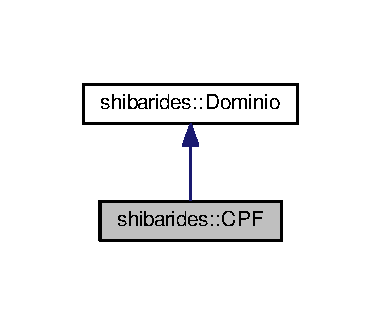
\includegraphics[width=183pt]{classshibarides_1_1CPF__inherit__graph}
\end{center}
\end{figure}


Diagrama de colaboração para shibarides\+:\+:C\+PF\+:\nopagebreak
\begin{figure}[H]
\begin{center}
\leavevmode
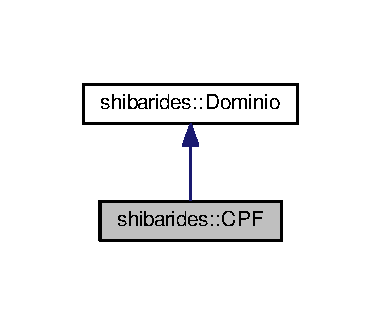
\includegraphics[width=183pt]{classshibarides_1_1CPF__coll__graph}
\end{center}
\end{figure}
\subsection*{Métodos Privados}
\begin{DoxyCompactItemize}
\item 
void \hyperlink{classshibarides_1_1CPF_a0764894456e73dde8130a07f95b68f08}{validate} (std\+::string)  throw (std\+::invalid\+\_\+argument)
\begin{DoxyCompactList}\small\item\em Função privada que define as regras de validação para o dominio. \end{DoxyCompactList}\end{DoxyCompactItemize}
\subsection*{Outros membros herdados}


\subsection{Métodos}
\index{shibarides\+::\+C\+PF@{shibarides\+::\+C\+PF}!validate@{validate}}
\index{validate@{validate}!shibarides\+::\+C\+PF@{shibarides\+::\+C\+PF}}
\subsubsection[{\texorpdfstring{validate(std\+::string)}{validate(std::string)}}]{\setlength{\rightskip}{0pt plus 5cm}void C\+P\+F\+::validate (
\begin{DoxyParamCaption}
\item[{std\+::string}]{}
\end{DoxyParamCaption}
) throw  std\+::invalid\+\_\+argument) \hspace{0.3cm}{\ttfamily [private]}, {\ttfamily [virtual]}}\hypertarget{classshibarides_1_1CPF_a0764894456e73dde8130a07f95b68f08}{}\label{classshibarides_1_1CPF_a0764894456e73dde8130a07f95b68f08}


Função privada que define as regras de validação para o dominio. 

Função pura abstrata, que é sobrescrita nos domínios e define o comportamento de cada domínio. Caso o valor passado nao seja valido, é lançada uma excessão std\+::invalid\+\_\+argument.


\begin{DoxyParams}{Parâmetros}
{\em string} & Valor a ser validado. \\
\hline
\end{DoxyParams}


Implementa \hyperlink{classshibarides_1_1Dominio_acc9445531455c072bbf708709aebbe55}{shibarides\+::\+Dominio}.



A documentação para esta classe foi gerada a partir dos seguintes arquivos\+:\begin{DoxyCompactItemize}
\item 
shibarides/Shiba\+Rides\+Domains.\+hpp\item 
shibarides/Shiba\+Rides\+Domains.\+cpp\end{DoxyCompactItemize}

\hypertarget{classshibarides_1_1Data}{}\section{Referência da Classe shibarides\+:\+:Data}
\label{classshibarides_1_1Data}\index{shibarides\+::\+Data@{shibarides\+::\+Data}}


\hyperlink{classshibarides_1_1Dominio}{Dominio} responsável pelas datas.  




{\ttfamily \#include $<$Shiba\+Rides\+Domains.\+hpp$>$}



Diagrama de Hierarquia para shibarides\+:\+:Data\+:\nopagebreak
\begin{figure}[H]
\begin{center}
\leavevmode
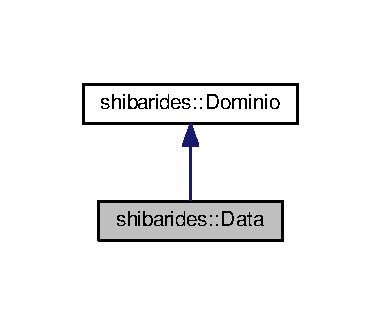
\includegraphics[width=183pt]{classshibarides_1_1Data__inherit__graph}
\end{center}
\end{figure}


Diagrama de colaboração para shibarides\+:\+:Data\+:\nopagebreak
\begin{figure}[H]
\begin{center}
\leavevmode
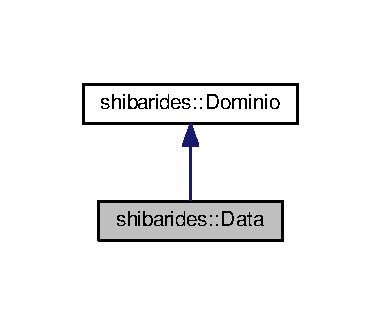
\includegraphics[width=183pt]{classshibarides_1_1Data__coll__graph}
\end{center}
\end{figure}
\subsection*{Métodos Privados}
\begin{DoxyCompactItemize}
\item 
void \hyperlink{classshibarides_1_1Data_a6240717eb60d01a7ab0c12336685c862}{validate} (std\+::string)  throw (std\+::invalid\+\_\+argument)
\begin{DoxyCompactList}\small\item\em Método que define as regras de validação para o dominio. \end{DoxyCompactList}\end{DoxyCompactItemize}
\subsection*{Outros membros herdados}


\subsection{Descrição Detalhada}
\hyperlink{classshibarides_1_1Dominio}{Dominio} responsável pelas datas. 

Representa as datas. Os valores permitidos seguem as seguintes regras\+: \begin{DoxyVerb}  Formato DD/MM/AAAA. DD é número de 1 e 31. MM é número de 1 e 12.
  AAAA é número de 2000 a 2099. A data deve considerar a ocorrência de
  anos bissextos.\end{DoxyVerb}
 

\subsection{Métodos}
\index{shibarides\+::\+Data@{shibarides\+::\+Data}!validate@{validate}}
\index{validate@{validate}!shibarides\+::\+Data@{shibarides\+::\+Data}}
\subsubsection[{\texorpdfstring{validate(std\+::string)}{validate(std::string)}}]{\setlength{\rightskip}{0pt plus 5cm}void Data\+::validate (
\begin{DoxyParamCaption}
\item[{std\+::string}]{value}
\end{DoxyParamCaption}
) throw  std\+::invalid\+\_\+argument) \hspace{0.3cm}{\ttfamily [private]}, {\ttfamily [virtual]}}\hypertarget{classshibarides_1_1Data_a6240717eb60d01a7ab0c12336685c862}{}\label{classshibarides_1_1Data_a6240717eb60d01a7ab0c12336685c862}


Método que define as regras de validação para o dominio. 

O método validate implementa as regras de validação para o dominio. Os valores permitidos seguem as seguintes regras\+:

Formato D\+D/\+M\+M/\+A\+A\+AA. DD é número de 1 e 31. MM é número de 1 e 12. A\+A\+AA é número de 2000 a 2099. A data deve considerar a ocorrência de anos bissextos.


\begin{DoxyParams}{Parâmetros}
{\em value} & Valor a ser validado \\
\hline
\end{DoxyParams}

\begin{DoxyExceptions}{Exceções}
{\em std\+::invalid\+\_\+argument} & Argumento invalido pelas regras do dominio \\
\hline
\end{DoxyExceptions}


Implementa \hyperlink{classshibarides_1_1Dominio_acc9445531455c072bbf708709aebbe55}{shibarides\+::\+Dominio}.



A documentação para esta classe foi gerada a partir dos seguintes arquivos\+:\begin{DoxyCompactItemize}
\item 
shibarides/Shiba\+Rides\+Domains.\+hpp\item 
shibarides/Shiba\+Rides\+Domains.\+cpp\end{DoxyCompactItemize}

\hypertarget{classshibarides_1_1Dominio}{}\section{Referência da Classe shibarides\+:\+:Dominio}
\label{classshibarides_1_1Dominio}\index{shibarides\+::\+Dominio@{shibarides\+::\+Dominio}}


Classe abstrata que serve de base para os domínios.  




{\ttfamily \#include $<$Shiba\+Rides\+Domains.\+hpp$>$}



Diagrama de Hierarquia para shibarides\+:\+:Dominio\+:
\nopagebreak
\begin{figure}[H]
\begin{center}
\leavevmode
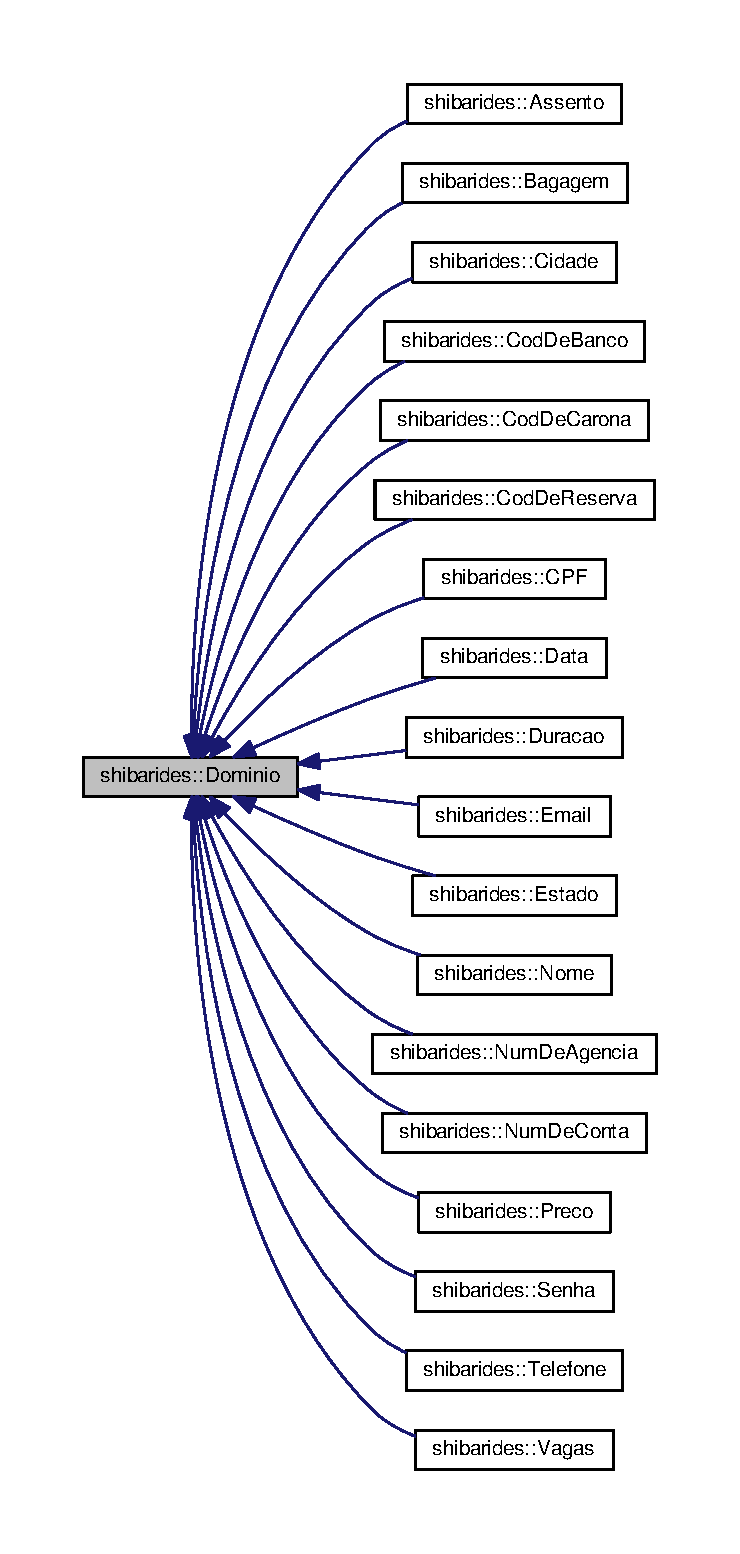
\includegraphics[height=550pt]{classshibarides_1_1Dominio__inherit__graph}
\end{center}
\end{figure}
\subsection*{Métodos Públicos}
\begin{DoxyCompactItemize}
\item 
\hyperlink{classshibarides_1_1Dominio_ab421ab3e3bcca7f47fe5320e0957b9a9}{Dominio} ()
\begin{DoxyCompactList}\small\item\em Construtor da classe \hyperlink{classshibarides_1_1Dominio}{Dominio}. \end{DoxyCompactList}\item 
void \hyperlink{classshibarides_1_1Dominio_a459a792e3f90b5b83880d3277c15747c}{set\+Value} (std\+::string)  throw (std\+::invalid\+\_\+argument)
\begin{DoxyCompactList}\small\item\em Armazena o valor passado, caso este seja valido para o dominio em questão. \end{DoxyCompactList}\item 
std\+::string \hyperlink{classshibarides_1_1Dominio_aa6fca113add7ee85dee788f4325fe564}{get\+Value} () const 
\begin{DoxyCompactList}\small\item\em Retorna o valor armazenado no campo value. \end{DoxyCompactList}\end{DoxyCompactItemize}
\subsection*{Métodos Privados}
\begin{DoxyCompactItemize}
\item 
virtual void \hyperlink{classshibarides_1_1Dominio_acc9445531455c072bbf708709aebbe55}{validate} (std\+::string)=0  throw (std\+::invalid\+\_\+argument)
\begin{DoxyCompactList}\small\item\em Função privada que define as regras de validação para o dominio. \end{DoxyCompactList}\end{DoxyCompactItemize}
\subsection*{Atributos Privados}
\begin{DoxyCompactItemize}
\item 
std\+::string \hyperlink{classshibarides_1_1Dominio_a840b839896c84528573c299496033dcc}{value}\hypertarget{classshibarides_1_1Dominio_a840b839896c84528573c299496033dcc}{}\label{classshibarides_1_1Dominio_a840b839896c84528573c299496033dcc}

\begin{DoxyCompactList}\small\item\em Armazena valores (todos os valores sao strings) \end{DoxyCompactList}\end{DoxyCompactItemize}


\subsection{Descrição Detalhada}
Classe abstrata que serve de base para os domínios. 

Classe da qual todos os dominios são herdados. Implementa as funçoes set\+Value e get\+Value, que servem para definir o valor armazenado em um dominio ou retornar esse valor. Todos os valores para os dominios sao armazenados na string value. É exigida a implementação da função abstrata pura validate em todos os dominios. Essa função define as regras pelas quais valores serao aceitos ou recusados pelo dominio. 

\subsection{Construtores \& Destrutores}
\index{shibarides\+::\+Dominio@{shibarides\+::\+Dominio}!Dominio@{Dominio}}
\index{Dominio@{Dominio}!shibarides\+::\+Dominio@{shibarides\+::\+Dominio}}
\subsubsection[{\texorpdfstring{Dominio()}{Dominio()}}]{\setlength{\rightskip}{0pt plus 5cm}Dominio\+::\+Dominio (
\begin{DoxyParamCaption}
{}
\end{DoxyParamCaption}
)}\hypertarget{classshibarides_1_1Dominio_ab421ab3e3bcca7f47fe5320e0957b9a9}{}\label{classshibarides_1_1Dominio_ab421ab3e3bcca7f47fe5320e0957b9a9}


Construtor da classe \hyperlink{classshibarides_1_1Dominio}{Dominio}. 

Apenas define o campo value como string vazia (\char`\"{}\char`\"{}) 

\subsection{Métodos}
\index{shibarides\+::\+Dominio@{shibarides\+::\+Dominio}!get\+Value@{get\+Value}}
\index{get\+Value@{get\+Value}!shibarides\+::\+Dominio@{shibarides\+::\+Dominio}}
\subsubsection[{\texorpdfstring{get\+Value() const }{getValue() const }}]{\setlength{\rightskip}{0pt plus 5cm}std\+::string Dominio\+::get\+Value (
\begin{DoxyParamCaption}
{}
\end{DoxyParamCaption}
) const}\hypertarget{classshibarides_1_1Dominio_aa6fca113add7ee85dee788f4325fe564}{}\label{classshibarides_1_1Dominio_aa6fca113add7ee85dee788f4325fe564}


Retorna o valor armazenado no campo value. 

A funçao get\+Value retorna o valor armazenado pelo dominio. Se o valor ainda nao tiver sido modificado, é retornada uma string vazia.

\begin{DoxyReturn}{Retorna}
string Valor armazenado pelo dominio 
\end{DoxyReturn}
\index{shibarides\+::\+Dominio@{shibarides\+::\+Dominio}!set\+Value@{set\+Value}}
\index{set\+Value@{set\+Value}!shibarides\+::\+Dominio@{shibarides\+::\+Dominio}}
\subsubsection[{\texorpdfstring{set\+Value(std\+::string)}{setValue(std::string)}}]{\setlength{\rightskip}{0pt plus 5cm}void Dominio\+::set\+Value (
\begin{DoxyParamCaption}
\item[{std\+::string}]{value}
\end{DoxyParamCaption}
) throw  std\+::invalid\+\_\+argument) }\hypertarget{classshibarides_1_1Dominio_a459a792e3f90b5b83880d3277c15747c}{}\label{classshibarides_1_1Dominio_a459a792e3f90b5b83880d3277c15747c}


Armazena o valor passado, caso este seja valido para o dominio em questão. 

A funçao set\+Value invoca o metodo validate do dominio, com o intuito de verificar se o valor passado é valido. Em caso positivo, o valor é armazenado no campo value do objeto. Em caso negativo, é lançada uma excessão do tipo std\+::invalid\+\_\+argument.


\begin{DoxyParams}{Parâmetros}
{\em value} & Valor a ser armazenado \\
\hline
\end{DoxyParams}
\index{shibarides\+::\+Dominio@{shibarides\+::\+Dominio}!validate@{validate}}
\index{validate@{validate}!shibarides\+::\+Dominio@{shibarides\+::\+Dominio}}
\subsubsection[{\texorpdfstring{validate(std\+::string)=0}{validate(std::string)=0}}]{\setlength{\rightskip}{0pt plus 5cm}virtual void shibarides\+::\+Dominio\+::validate (
\begin{DoxyParamCaption}
\item[{std\+::string}]{}
\end{DoxyParamCaption}
) throw  std\+::invalid\+\_\+argument) \hspace{0.3cm}{\ttfamily [private]}, {\ttfamily [pure virtual]}}\hypertarget{classshibarides_1_1Dominio_acc9445531455c072bbf708709aebbe55}{}\label{classshibarides_1_1Dominio_acc9445531455c072bbf708709aebbe55}


Função privada que define as regras de validação para o dominio. 

Função pura abstrata, que é sobrescrita nos domínios e define o comportamento de cada domínio. Caso o valor passado nao seja valido, é lançada uma excessão std\+::invalid\+\_\+argument.


\begin{DoxyParams}{Parâmetros}
{\em string} & Valor a ser validado. \\
\hline
\end{DoxyParams}


Implementado por \hyperlink{classshibarides_1_1Vagas_ae5f73c52819397524b0334d9e609d296}{shibarides\+::\+Vagas}, \hyperlink{classshibarides_1_1Senha_a733550b46c79a95df9f5f4163f0be923}{shibarides\+::\+Senha}, \hyperlink{classshibarides_1_1Telefone_aa798f740a30faef8d2599950284ded33}{shibarides\+::\+Telefone}, \hyperlink{classshibarides_1_1Preco_ae57d286adf4db4b1132001f8736892f7}{shibarides\+::\+Preco}, \hyperlink{classshibarides_1_1NumDeConta_afe1c1bfd98ca97d59b521a6e7ac9d5ef}{shibarides\+::\+Num\+De\+Conta}, \hyperlink{classshibarides_1_1NumDeAgencia_a4bf7dd9204aff60838faf4f2362d8c3b}{shibarides\+::\+Num\+De\+Agencia}, \hyperlink{classshibarides_1_1Nome_aae6c1656422424a675e79a03a7ca534e}{shibarides\+::\+Nome}, \hyperlink{classshibarides_1_1Email_a0589d5dedd6e072f454391cd2e2873ee}{shibarides\+::\+Email}, \hyperlink{classshibarides_1_1Estado_a87dff745c1b1f487eae4bd4461e8a1ef}{shibarides\+::\+Estado}, \hyperlink{classshibarides_1_1Duracao_aa64196edbfe284120c3d498e20212a99}{shibarides\+::\+Duracao}, \hyperlink{classshibarides_1_1Data_a6240717eb60d01a7ab0c12336685c862}{shibarides\+::\+Data}, \hyperlink{classshibarides_1_1CPF_a0764894456e73dde8130a07f95b68f08}{shibarides\+::\+C\+PF}, \hyperlink{classshibarides_1_1Cidade_a2a2455d16a0d316ebcc57c4389e1a0b0}{shibarides\+::\+Cidade}, \hyperlink{classshibarides_1_1CodDeReserva_a595a667ca295b1adc5eedefd773d8027}{shibarides\+::\+Cod\+De\+Reserva}, \hyperlink{classshibarides_1_1CodDeCarona_a2713cdc938576b30a6f7e59ddc67a848}{shibarides\+::\+Cod\+De\+Carona}, \hyperlink{classshibarides_1_1CodDeBanco_a111bd50227f559d36010ddbf7bee1107}{shibarides\+::\+Cod\+De\+Banco}, \hyperlink{classshibarides_1_1Bagagem_aad85c0b035f3f3202130160edc35d41d}{shibarides\+::\+Bagagem} e \hyperlink{classshibarides_1_1Assento_a8a2099562808c49caff59569bcb977c3}{shibarides\+::\+Assento}.



A documentação para esta classe foi gerada a partir dos seguintes arquivos\+:\begin{DoxyCompactItemize}
\item 
shibarides/Shiba\+Rides\+Domains.\+hpp\item 
shibarides/Shiba\+Rides\+Domains.\+cpp\end{DoxyCompactItemize}

\hypertarget{classshibarides_1_1Duracao}{}\section{Referência da Classe shibarides\+:\+:Duracao}
\label{classshibarides_1_1Duracao}\index{shibarides\+::\+Duracao@{shibarides\+::\+Duracao}}


\hyperlink{classshibarides_1_1Dominio}{Dominio} responsável pela duração das viagens.  




{\ttfamily \#include $<$Shiba\+Rides\+Domains.\+hpp$>$}



Diagrama de Hierarquia para shibarides\+:\+:Duracao\+:\nopagebreak
\begin{figure}[H]
\begin{center}
\leavevmode
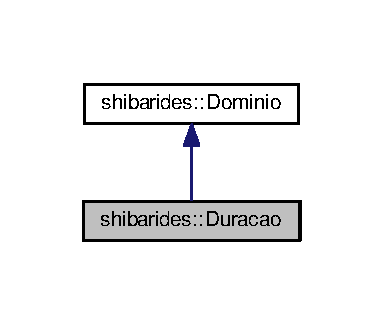
\includegraphics[width=184pt]{classshibarides_1_1Duracao__inherit__graph}
\end{center}
\end{figure}


Diagrama de colaboração para shibarides\+:\+:Duracao\+:\nopagebreak
\begin{figure}[H]
\begin{center}
\leavevmode
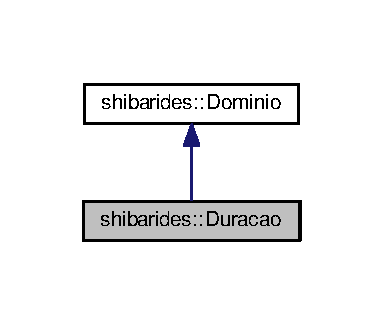
\includegraphics[width=184pt]{classshibarides_1_1Duracao__coll__graph}
\end{center}
\end{figure}
\subsection*{Métodos Privados}
\begin{DoxyCompactItemize}
\item 
void \hyperlink{classshibarides_1_1Duracao_aa64196edbfe284120c3d498e20212a99}{validate} (std\+::string)  throw (std\+::invalid\+\_\+argument)
\begin{DoxyCompactList}\small\item\em Método que define as regras de validação para o dominio. \end{DoxyCompactList}\end{DoxyCompactItemize}
\subsection*{Outros membros herdados}


\subsection{Descrição Detalhada}
\hyperlink{classshibarides_1_1Dominio}{Dominio} responsável pela duração das viagens. 

Representa a duração das viagens. Os valores permitidos são representados em horas, podendo ser de 1 a 48. 

\subsection{Métodos}
\index{shibarides\+::\+Duracao@{shibarides\+::\+Duracao}!validate@{validate}}
\index{validate@{validate}!shibarides\+::\+Duracao@{shibarides\+::\+Duracao}}
\subsubsection[{\texorpdfstring{validate(std\+::string)}{validate(std::string)}}]{\setlength{\rightskip}{0pt plus 5cm}void Duracao\+::validate (
\begin{DoxyParamCaption}
\item[{std\+::string}]{value}
\end{DoxyParamCaption}
) throw  std\+::invalid\+\_\+argument) \hspace{0.3cm}{\ttfamily [private]}, {\ttfamily [virtual]}}\hypertarget{classshibarides_1_1Duracao_aa64196edbfe284120c3d498e20212a99}{}\label{classshibarides_1_1Duracao_aa64196edbfe284120c3d498e20212a99}


Método que define as regras de validação para o dominio. 

O método validate implementa as regras de validação para o dominio. Os valores permitidos são representados em horas, podendo ser de 1 a 48.


\begin{DoxyParams}{Parâmetros}
{\em value} & Valor a ser validado \\
\hline
\end{DoxyParams}

\begin{DoxyExceptions}{Exceções}
{\em std\+::invalid\+\_\+argument} & Argumento invalido pelas regras do dominio \\
\hline
\end{DoxyExceptions}


Implementa \hyperlink{classshibarides_1_1Dominio_acc9445531455c072bbf708709aebbe55}{shibarides\+::\+Dominio}.



A documentação para esta classe foi gerada a partir dos seguintes arquivos\+:\begin{DoxyCompactItemize}
\item 
shibarides/domains/Shiba\+Rides\+Domains.\+hpp\item 
shibarides/domains/Shiba\+Rides\+Domains.\+cpp\end{DoxyCompactItemize}

\hypertarget{classshibarides_1_1Email}{}\section{Referência da Classe shibarides\+:\+:Email}
\label{classshibarides_1_1Email}\index{shibarides\+::\+Email@{shibarides\+::\+Email}}


Diagrama de Hierarquia para shibarides\+:\+:Email\+:\nopagebreak
\begin{figure}[H]
\begin{center}
\leavevmode
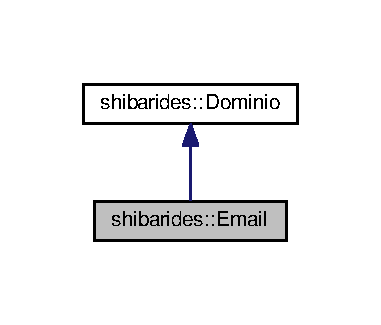
\includegraphics[width=183pt]{classshibarides_1_1Email__inherit__graph}
\end{center}
\end{figure}


Diagrama de colaboração para shibarides\+:\+:Email\+:\nopagebreak
\begin{figure}[H]
\begin{center}
\leavevmode
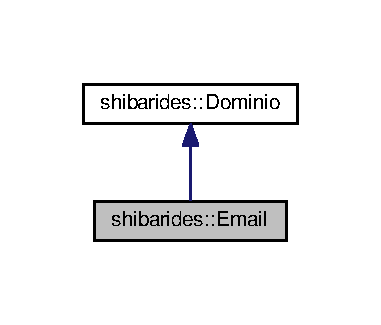
\includegraphics[width=183pt]{classshibarides_1_1Email__coll__graph}
\end{center}
\end{figure}
\subsection*{Métodos Privados}
\begin{DoxyCompactItemize}
\item 
void \hyperlink{classshibarides_1_1Email_a0589d5dedd6e072f454391cd2e2873ee}{validate} (std\+::string)  throw (std\+::invalid\+\_\+argument)
\begin{DoxyCompactList}\small\item\em Função privada que define as regras de validação para o dominio. \end{DoxyCompactList}\end{DoxyCompactItemize}
\subsection*{Outros membros herdados}


\subsection{Métodos}
\index{shibarides\+::\+Email@{shibarides\+::\+Email}!validate@{validate}}
\index{validate@{validate}!shibarides\+::\+Email@{shibarides\+::\+Email}}
\subsubsection[{\texorpdfstring{validate(std\+::string)}{validate(std::string)}}]{\setlength{\rightskip}{0pt plus 5cm}void Email\+::validate (
\begin{DoxyParamCaption}
\item[{std\+::string}]{}
\end{DoxyParamCaption}
) throw  std\+::invalid\+\_\+argument) \hspace{0.3cm}{\ttfamily [private]}, {\ttfamily [virtual]}}\hypertarget{classshibarides_1_1Email_a0589d5dedd6e072f454391cd2e2873ee}{}\label{classshibarides_1_1Email_a0589d5dedd6e072f454391cd2e2873ee}


Função privada que define as regras de validação para o dominio. 

Função pura abstrata, que é sobrescrita nos domínios e define o comportamento de cada domínio. Caso o valor passado nao seja valido, é lançada uma excessão std\+::invalid\+\_\+argument.


\begin{DoxyParams}{Parâmetros}
{\em string} & Valor a ser validado. \\
\hline
\end{DoxyParams}


Implementa \hyperlink{classshibarides_1_1Dominio_acc9445531455c072bbf708709aebbe55}{shibarides\+::\+Dominio}.



A documentação para esta classe foi gerada a partir dos seguintes arquivos\+:\begin{DoxyCompactItemize}
\item 
shibarides/Shiba\+Rides\+Domains.\+hpp\item 
shibarides/Shiba\+Rides\+Domains.\+cpp\end{DoxyCompactItemize}

\hypertarget{classshibarides_1_1Estado}{}\section{Referência da Classe shibarides\+:\+:Estado}
\label{classshibarides_1_1Estado}\index{shibarides\+::\+Estado@{shibarides\+::\+Estado}}


\hyperlink{classshibarides_1_1Dominio}{Dominio} responsável pelos estados de origem e destino das viagens.  




{\ttfamily \#include $<$Shiba\+Rides\+Domains.\+hpp$>$}



Diagrama de Hierarquia para shibarides\+:\+:Estado\+:\nopagebreak
\begin{figure}[H]
\begin{center}
\leavevmode
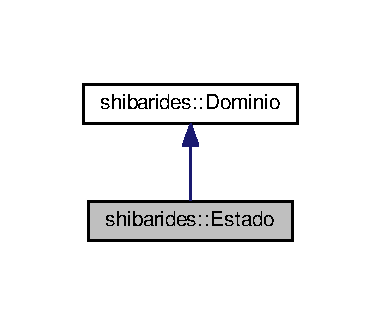
\includegraphics[width=183pt]{classshibarides_1_1Estado__inherit__graph}
\end{center}
\end{figure}


Diagrama de colaboração para shibarides\+:\+:Estado\+:\nopagebreak
\begin{figure}[H]
\begin{center}
\leavevmode
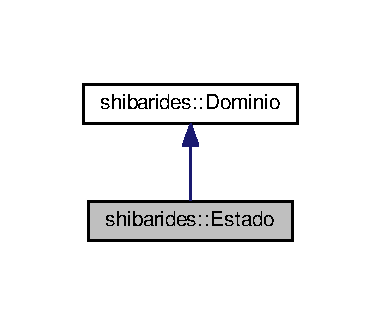
\includegraphics[width=183pt]{classshibarides_1_1Estado__coll__graph}
\end{center}
\end{figure}
\subsection*{Métodos Privados}
\begin{DoxyCompactItemize}
\item 
void \hyperlink{classshibarides_1_1Estado_a87dff745c1b1f487eae4bd4461e8a1ef}{validate} (std\+::string)  throw (std\+::invalid\+\_\+argument)
\begin{DoxyCompactList}\small\item\em Método que define as regras de validação para o dominio. \end{DoxyCompactList}\end{DoxyCompactItemize}
\subsection*{Outros membros herdados}


\subsection{Descrição Detalhada}
\hyperlink{classshibarides_1_1Dominio}{Dominio} responsável pelos estados de origem e destino das viagens. 

Representa os estados nas caronas. Os valores permitidos são representados em siglas para cada estado, e podem ser qualquer estado brasileiro. 

\subsection{Métodos}
\index{shibarides\+::\+Estado@{shibarides\+::\+Estado}!validate@{validate}}
\index{validate@{validate}!shibarides\+::\+Estado@{shibarides\+::\+Estado}}
\subsubsection[{\texorpdfstring{validate(std\+::string)}{validate(std::string)}}]{\setlength{\rightskip}{0pt plus 5cm}void Estado\+::validate (
\begin{DoxyParamCaption}
\item[{std\+::string}]{value}
\end{DoxyParamCaption}
) throw  std\+::invalid\+\_\+argument) \hspace{0.3cm}{\ttfamily [private]}, {\ttfamily [virtual]}}\hypertarget{classshibarides_1_1Estado_a87dff745c1b1f487eae4bd4461e8a1ef}{}\label{classshibarides_1_1Estado_a87dff745c1b1f487eae4bd4461e8a1ef}


Método que define as regras de validação para o dominio. 

O método validate implementa as regras de validação para o dominio. Os valores permitidos são representados em siglas para cada estado, e podem ser qualquer estado brasileiro\+: AC, AL, AP, AM, BA, CE, DF, ES, GO, MA, MT, MS, MG, PA, PB, PR, PE, PI, RJ, RN, RS, RO, RR, SC, SP, SE, TO


\begin{DoxyParams}{Parâmetros}
{\em value} & Valor a ser validado \\
\hline
\end{DoxyParams}

\begin{DoxyExceptions}{Exceções}
{\em std\+::invalid\+\_\+argument} & Argumento invalido pelas regras do dominio \\
\hline
\end{DoxyExceptions}


Implementa \hyperlink{classshibarides_1_1Dominio_acc9445531455c072bbf708709aebbe55}{shibarides\+::\+Dominio}.



A documentação para esta classe foi gerada a partir dos seguintes arquivos\+:\begin{DoxyCompactItemize}
\item 
shibarides/Shiba\+Rides\+Domains.\+hpp\item 
shibarides/Shiba\+Rides\+Domains.\+cpp\end{DoxyCompactItemize}

\hypertarget{classshibarides_1_1Nome}{}\section{Referência da Classe shibarides\+:\+:Nome}
\label{classshibarides_1_1Nome}\index{shibarides\+::\+Nome@{shibarides\+::\+Nome}}


\hyperlink{classshibarides_1_1Dominio}{Dominio} responsável pela validação dos nomes de usuario.  




{\ttfamily \#include $<$Shiba\+Rides\+Domains.\+hpp$>$}



Diagrama de Hierarquia para shibarides\+:\+:Nome\+:\nopagebreak
\begin{figure}[H]
\begin{center}
\leavevmode
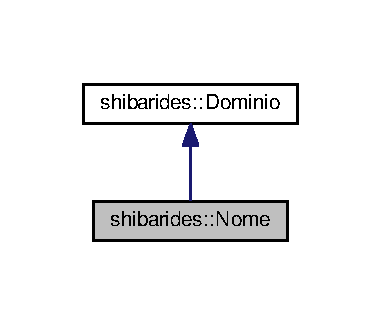
\includegraphics[width=183pt]{classshibarides_1_1Nome__inherit__graph}
\end{center}
\end{figure}


Diagrama de colaboração para shibarides\+:\+:Nome\+:\nopagebreak
\begin{figure}[H]
\begin{center}
\leavevmode
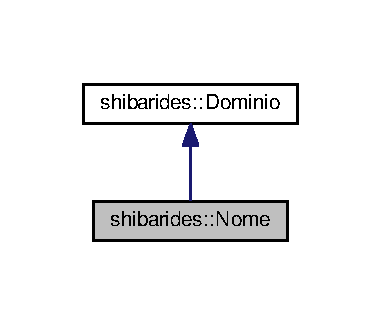
\includegraphics[width=183pt]{classshibarides_1_1Nome__coll__graph}
\end{center}
\end{figure}
\subsection*{Métodos Privados}
\begin{DoxyCompactItemize}
\item 
void \hyperlink{classshibarides_1_1Nome_aae6c1656422424a675e79a03a7ca534e}{validate} (std\+::string)  throw (std\+::invalid\+\_\+argument)
\begin{DoxyCompactList}\small\item\em Método que define as regras de validação para o dominio. \end{DoxyCompactList}\end{DoxyCompactItemize}
\subsection*{Outros membros herdados}


\subsection{Descrição Detalhada}
\hyperlink{classshibarides_1_1Dominio}{Dominio} responsável pela validação dos nomes de usuario. 

Representa os Nomes dos usuarios. 

\subsection{Métodos}
\index{shibarides\+::\+Nome@{shibarides\+::\+Nome}!validate@{validate}}
\index{validate@{validate}!shibarides\+::\+Nome@{shibarides\+::\+Nome}}
\subsubsection[{\texorpdfstring{validate(std\+::string)}{validate(std::string)}}]{\setlength{\rightskip}{0pt plus 5cm}void Nome\+::validate (
\begin{DoxyParamCaption}
\item[{std\+::string}]{value}
\end{DoxyParamCaption}
) throw  std\+::invalid\+\_\+argument) \hspace{0.3cm}{\ttfamily [private]}, {\ttfamily [virtual]}}\hypertarget{classshibarides_1_1Nome_aae6c1656422424a675e79a03a7ca534e}{}\label{classshibarides_1_1Nome_aae6c1656422424a675e79a03a7ca534e}


Método que define as regras de validação para o dominio. 

O método validate implementa as regras de validação para o dominio. Os valores permitidos seguem as seguintes regras\+:

De 1 a 20 caracteres, onde cada caracter pode ser letra, ponto ou espaço. Pelo menos um caracter é letra, antes de ponto deve haver letra e não há espaços em sequência.


\begin{DoxyParams}{Parâmetros}
{\em value} & Valor a ser validado \\
\hline
\end{DoxyParams}

\begin{DoxyExceptions}{Exceções}
{\em std\+::invalid\+\_\+argument} & Argumento invalido pelas regras do dominio \\
\hline
\end{DoxyExceptions}


Implementa \hyperlink{classshibarides_1_1Dominio_acc9445531455c072bbf708709aebbe55}{shibarides\+::\+Dominio}.



A documentação para esta classe foi gerada a partir dos seguintes arquivos\+:\begin{DoxyCompactItemize}
\item 
shibarides/domains/Shiba\+Rides\+Domains.\+hpp\item 
shibarides/domains/Shiba\+Rides\+Domains.\+cpp\end{DoxyCompactItemize}

\hypertarget{classshibarides_1_1NumDeAgencia}{}\section{Referência da Classe shibarides\+:\+:Num\+De\+Agencia}
\label{classshibarides_1_1NumDeAgencia}\index{shibarides\+::\+Num\+De\+Agencia@{shibarides\+::\+Num\+De\+Agencia}}


Diagrama de Hierarquia para shibarides\+:\+:Num\+De\+Agencia\+:\nopagebreak
\begin{figure}[H]
\begin{center}
\leavevmode
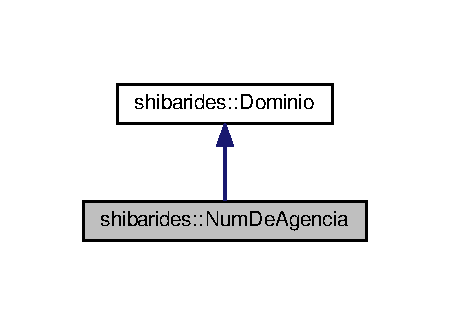
\includegraphics[width=216pt]{classshibarides_1_1NumDeAgencia__inherit__graph}
\end{center}
\end{figure}


Diagrama de colaboração para shibarides\+:\+:Num\+De\+Agencia\+:\nopagebreak
\begin{figure}[H]
\begin{center}
\leavevmode
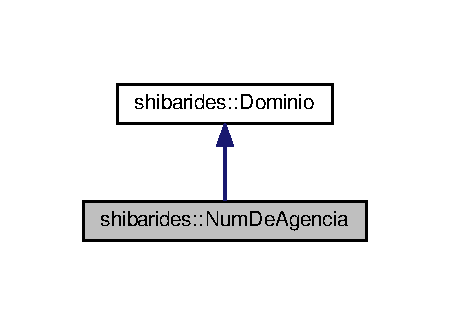
\includegraphics[width=216pt]{classshibarides_1_1NumDeAgencia__coll__graph}
\end{center}
\end{figure}
\subsection*{Outros membros herdados}


A documentação para esta classe foi gerada a partir dos seguintes arquivos\+:\begin{DoxyCompactItemize}
\item 
shibarides/Shiba\+Rides\+Domains.\+hpp\item 
shibarides/Shiba\+Rides\+Domains.\+cpp\end{DoxyCompactItemize}

\hypertarget{classshibarides_1_1NumDeConta}{}\section{Referência da Classe shibarides\+:\+:Num\+De\+Conta}
\label{classshibarides_1_1NumDeConta}\index{shibarides\+::\+Num\+De\+Conta@{shibarides\+::\+Num\+De\+Conta}}


Diagrama de Hierarquia para shibarides\+:\+:Num\+De\+Conta\+:
% FIG 0


Diagrama de colaboração para shibarides\+:\+:Num\+De\+Conta\+:
% FIG 1
\subsection*{Outros membros herdados}


A documentação para esta classe foi gerada a partir dos seguintes arquivos\+:\begin{DoxyCompactItemize}
\item 
shibarides/Shiba\+Rides\+Domains.\+hpp\item 
shibarides/Shiba\+Rides\+Domains.\+cpp\end{DoxyCompactItemize}

\hypertarget{classshibarides_1_1Preco}{}\section{Referência da Classe shibarides\+:\+:Preco}
\label{classshibarides_1_1Preco}\index{shibarides\+::\+Preco@{shibarides\+::\+Preco}}


Diagrama de Hierarquia para shibarides\+:\+:Preco\+:\nopagebreak
\begin{figure}[H]
\begin{center}
\leavevmode
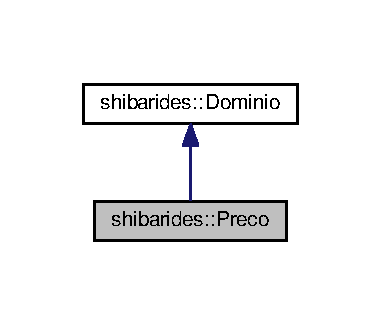
\includegraphics[width=183pt]{classshibarides_1_1Preco__inherit__graph}
\end{center}
\end{figure}


Diagrama de colaboração para shibarides\+:\+:Preco\+:\nopagebreak
\begin{figure}[H]
\begin{center}
\leavevmode
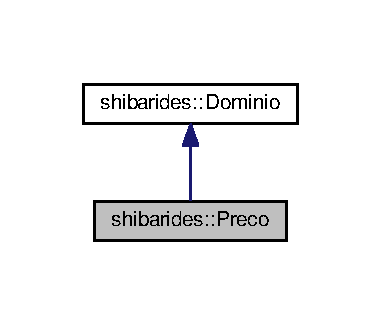
\includegraphics[width=183pt]{classshibarides_1_1Preco__coll__graph}
\end{center}
\end{figure}
\subsection*{Outros membros herdados}


A documentação para esta classe foi gerada a partir dos seguintes arquivos\+:\begin{DoxyCompactItemize}
\item 
shibarides/Shiba\+Rides\+Domains.\+hpp\item 
shibarides/Shiba\+Rides\+Domains.\+cpp\end{DoxyCompactItemize}

\hypertarget{classshibarides_1_1Reserva}{}\section{Referência da Classe shibarides\+:\+:Reserva}
\label{classshibarides_1_1Reserva}\index{shibarides\+::\+Reserva@{shibarides\+::\+Reserva}}


Diagrama de colaboração para shibarides\+:\+:Reserva\+:\nopagebreak
\begin{figure}[H]
\begin{center}
\leavevmode
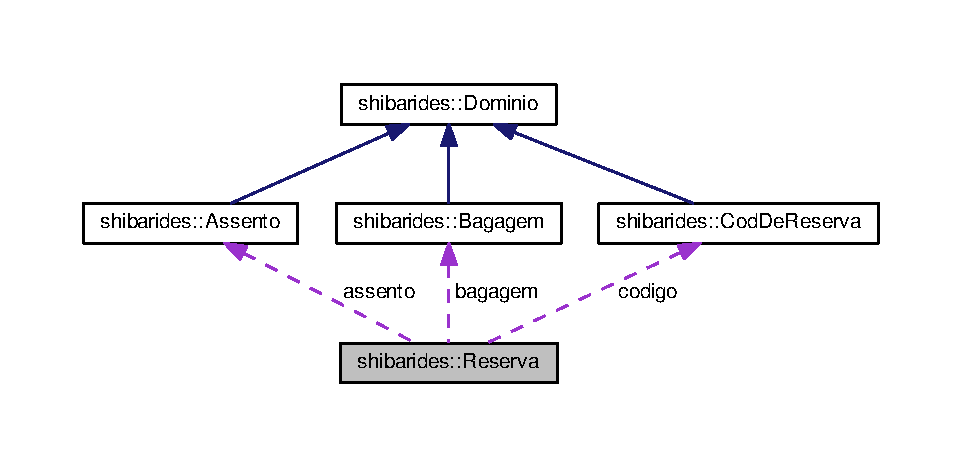
\includegraphics[width=350pt]{classshibarides_1_1Reserva__coll__graph}
\end{center}
\end{figure}
\subsection*{Métodos Públicos}
\begin{DoxyCompactItemize}
\item 
void {\bfseries set\+Codigo} (const \hyperlink{classshibarides_1_1CodDeReserva}{Cod\+De\+Reserva} \&codigo)\hypertarget{classshibarides_1_1Reserva_a8f2e70e8f8e6a0b739731c3ddaca1e2f}{}\label{classshibarides_1_1Reserva_a8f2e70e8f8e6a0b739731c3ddaca1e2f}

\item 
\hyperlink{classshibarides_1_1CodDeReserva}{Cod\+De\+Reserva} {\bfseries get\+Codigo} () const \hypertarget{classshibarides_1_1Reserva_a707e6f4248e3ee1ed8f0c1e3893c834d}{}\label{classshibarides_1_1Reserva_a707e6f4248e3ee1ed8f0c1e3893c834d}

\item 
void {\bfseries set\+Assento} (const \hyperlink{classshibarides_1_1Assento}{Assento} \&assento)\hypertarget{classshibarides_1_1Reserva_a9013c5f1d6638ccc77e4a37071409d9b}{}\label{classshibarides_1_1Reserva_a9013c5f1d6638ccc77e4a37071409d9b}

\item 
\hyperlink{classshibarides_1_1Assento}{Assento} {\bfseries get\+Assento} () const \hypertarget{classshibarides_1_1Reserva_a9a2c89b1c70b8ad4dc8124a229c5c8ca}{}\label{classshibarides_1_1Reserva_a9a2c89b1c70b8ad4dc8124a229c5c8ca}

\item 
void {\bfseries set\+Bagagem} (const \hyperlink{classshibarides_1_1Bagagem}{Bagagem} \&bagagem)\hypertarget{classshibarides_1_1Reserva_aaef804b78d7ae0979d38625f29ee7a09}{}\label{classshibarides_1_1Reserva_aaef804b78d7ae0979d38625f29ee7a09}

\item 
\hyperlink{classshibarides_1_1Bagagem}{Bagagem} {\bfseries get\+Bagagem} () const \hypertarget{classshibarides_1_1Reserva_a427286c7b59a6cf0ea17bd9cb8165139}{}\label{classshibarides_1_1Reserva_a427286c7b59a6cf0ea17bd9cb8165139}

\end{DoxyCompactItemize}
\subsection*{Atributos Privados}
\begin{DoxyCompactItemize}
\item 
\hyperlink{classshibarides_1_1CodDeReserva}{Cod\+De\+Reserva} {\bfseries codigo}\hypertarget{classshibarides_1_1Reserva_a2f7eaae7c2f5378ff302d5ae2b5fbb40}{}\label{classshibarides_1_1Reserva_a2f7eaae7c2f5378ff302d5ae2b5fbb40}

\item 
\hyperlink{classshibarides_1_1Assento}{Assento} {\bfseries assento}\hypertarget{classshibarides_1_1Reserva_a7d97d0663be20fdcf657163c5a6d080c}{}\label{classshibarides_1_1Reserva_a7d97d0663be20fdcf657163c5a6d080c}

\item 
\hyperlink{classshibarides_1_1Bagagem}{Bagagem} {\bfseries bagagem}\hypertarget{classshibarides_1_1Reserva_a1f432400419baf386812117ce49990e6}{}\label{classshibarides_1_1Reserva_a1f432400419baf386812117ce49990e6}

\end{DoxyCompactItemize}


A documentação para esta classe foi gerada a partir do seguinte arquivo\+:\begin{DoxyCompactItemize}
\item 
shibarides/Shiba\+Rides\+Entities.\+hpp\end{DoxyCompactItemize}

\hypertarget{classshibarides_1_1Senha}{}\section{Referência da Classe shibarides\+:\+:Senha}
\label{classshibarides_1_1Senha}\index{shibarides\+::\+Senha@{shibarides\+::\+Senha}}


Diagrama de Hierarquia para shibarides\+:\+:Senha\+:\nopagebreak
\begin{figure}[H]
\begin{center}
\leavevmode
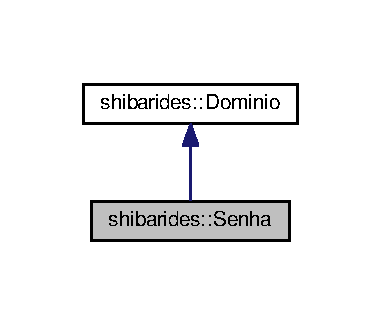
\includegraphics[width=183pt]{classshibarides_1_1Senha__inherit__graph}
\end{center}
\end{figure}


Diagrama de colaboração para shibarides\+:\+:Senha\+:\nopagebreak
\begin{figure}[H]
\begin{center}
\leavevmode
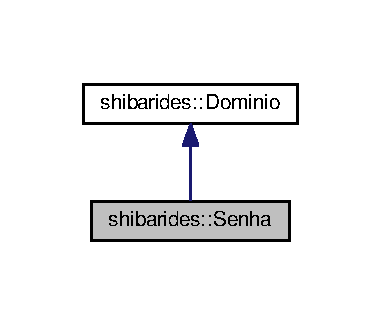
\includegraphics[width=183pt]{classshibarides_1_1Senha__coll__graph}
\end{center}
\end{figure}
\subsection*{Métodos Privados}
\begin{DoxyCompactItemize}
\item 
void \hyperlink{classshibarides_1_1Senha_a733550b46c79a95df9f5f4163f0be923}{validate} (std\+::string)  throw (std\+::invalid\+\_\+argument)
\begin{DoxyCompactList}\small\item\em Função privada que define as regras de validação para o dominio. \end{DoxyCompactList}\end{DoxyCompactItemize}
\subsection*{Outros membros herdados}


\subsection{Métodos}
\index{shibarides\+::\+Senha@{shibarides\+::\+Senha}!validate@{validate}}
\index{validate@{validate}!shibarides\+::\+Senha@{shibarides\+::\+Senha}}
\subsubsection[{\texorpdfstring{validate(std\+::string)}{validate(std::string)}}]{\setlength{\rightskip}{0pt plus 5cm}void Senha\+::validate (
\begin{DoxyParamCaption}
\item[{std\+::string}]{}
\end{DoxyParamCaption}
) throw  std\+::invalid\+\_\+argument) \hspace{0.3cm}{\ttfamily [private]}, {\ttfamily [virtual]}}\hypertarget{classshibarides_1_1Senha_a733550b46c79a95df9f5f4163f0be923}{}\label{classshibarides_1_1Senha_a733550b46c79a95df9f5f4163f0be923}


Função privada que define as regras de validação para o dominio. 

Função pura abstrata, que é sobrescrita nos domínios e define o comportamento de cada domínio. Caso o valor passado nao seja valido, é lançada uma excessão std\+::invalid\+\_\+argument.


\begin{DoxyParams}{Parâmetros}
{\em string} & Valor a ser validado. \\
\hline
\end{DoxyParams}


Implementa \hyperlink{classshibarides_1_1Dominio_acc9445531455c072bbf708709aebbe55}{shibarides\+::\+Dominio}.



A documentação para esta classe foi gerada a partir dos seguintes arquivos\+:\begin{DoxyCompactItemize}
\item 
shibarides/Shiba\+Rides\+Domains.\+hpp\item 
shibarides/Shiba\+Rides\+Domains.\+cpp\end{DoxyCompactItemize}

\hypertarget{classshibarides_1_1Telefone}{}\section{Referência da Classe shibarides\+:\+:Telefone}
\label{classshibarides_1_1Telefone}\index{shibarides\+::\+Telefone@{shibarides\+::\+Telefone}}


Diagrama de Hierarquia para shibarides\+:\+:Telefone\+:\nopagebreak
\begin{figure}[H]
\begin{center}
\leavevmode
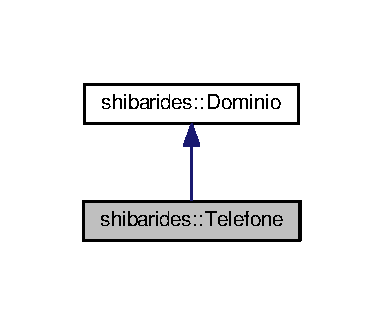
\includegraphics[width=184pt]{classshibarides_1_1Telefone__inherit__graph}
\end{center}
\end{figure}


Diagrama de colaboração para shibarides\+:\+:Telefone\+:\nopagebreak
\begin{figure}[H]
\begin{center}
\leavevmode
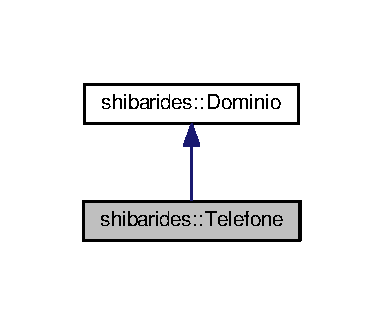
\includegraphics[width=184pt]{classshibarides_1_1Telefone__coll__graph}
\end{center}
\end{figure}
\subsection*{Métodos Privados}
\begin{DoxyCompactItemize}
\item 
void \hyperlink{classshibarides_1_1Telefone_aa798f740a30faef8d2599950284ded33}{validate} (std\+::string)  throw (std\+::invalid\+\_\+argument)
\begin{DoxyCompactList}\small\item\em Função privada que define as regras de validação para o dominio. \end{DoxyCompactList}\end{DoxyCompactItemize}
\subsection*{Outros membros herdados}


\subsection{Métodos}
\index{shibarides\+::\+Telefone@{shibarides\+::\+Telefone}!validate@{validate}}
\index{validate@{validate}!shibarides\+::\+Telefone@{shibarides\+::\+Telefone}}
\subsubsection[{\texorpdfstring{validate(std\+::string)}{validate(std::string)}}]{\setlength{\rightskip}{0pt plus 5cm}void Telefone\+::validate (
\begin{DoxyParamCaption}
\item[{std\+::string}]{}
\end{DoxyParamCaption}
) throw  std\+::invalid\+\_\+argument) \hspace{0.3cm}{\ttfamily [private]}, {\ttfamily [virtual]}}\hypertarget{classshibarides_1_1Telefone_aa798f740a30faef8d2599950284ded33}{}\label{classshibarides_1_1Telefone_aa798f740a30faef8d2599950284ded33}


Função privada que define as regras de validação para o dominio. 

Função pura abstrata, que é sobrescrita nos domínios e define o comportamento de cada domínio. Caso o valor passado nao seja valido, é lançada uma excessão std\+::invalid\+\_\+argument.


\begin{DoxyParams}{Parâmetros}
{\em string} & Valor a ser validado. \\
\hline
\end{DoxyParams}


Implementa \hyperlink{classshibarides_1_1Dominio_acc9445531455c072bbf708709aebbe55}{shibarides\+::\+Dominio}.



A documentação para esta classe foi gerada a partir dos seguintes arquivos\+:\begin{DoxyCompactItemize}
\item 
shibarides/Shiba\+Rides\+Domains.\+hpp\item 
shibarides/Shiba\+Rides\+Domains.\+cpp\end{DoxyCompactItemize}

\hypertarget{classshibarides_1_1TUAssento}{}\section{Referência da Classe shibarides\+:\+:T\+U\+Assento}
\label{classshibarides_1_1TUAssento}\index{shibarides\+::\+T\+U\+Assento@{shibarides\+::\+T\+U\+Assento}}


Diagrama de Hierarquia para shibarides\+:\+:T\+U\+Assento\+:\nopagebreak
\begin{figure}[H]
\begin{center}
\leavevmode
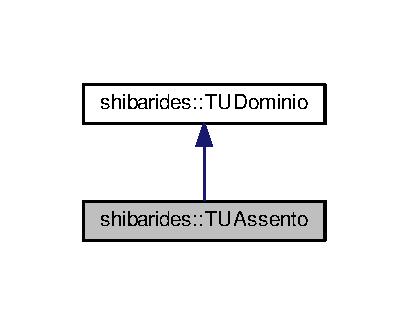
\includegraphics[width=196pt]{classshibarides_1_1TUAssento__inherit__graph}
\end{center}
\end{figure}


Diagrama de colaboração para shibarides\+:\+:T\+U\+Assento\+:\nopagebreak
\begin{figure}[H]
\begin{center}
\leavevmode
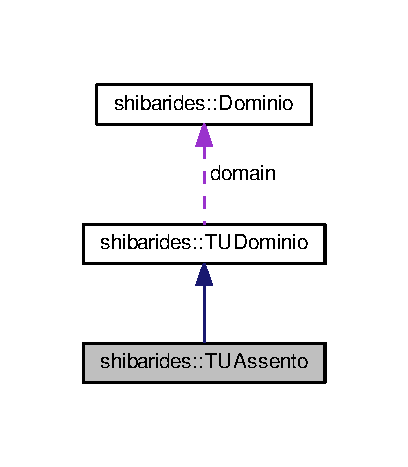
\includegraphics[width=196pt]{classshibarides_1_1TUAssento__coll__graph}
\end{center}
\end{figure}
\subsection*{Métodos Privados}
\begin{DoxyCompactItemize}
\item 
void {\bfseries gen\+Fail\+Values} ()\hypertarget{classshibarides_1_1TUAssento_a89408b642e71a79865b50f649c7db953}{}\label{classshibarides_1_1TUAssento_a89408b642e71a79865b50f649c7db953}

\item 
void {\bfseries gen\+Success\+Values} ()\hypertarget{classshibarides_1_1TUAssento_a92cebd28fdf14165b5a6492df3dd2619}{}\label{classshibarides_1_1TUAssento_a92cebd28fdf14165b5a6492df3dd2619}

\item 
void {\bfseries create\+Domain} ()\hypertarget{classshibarides_1_1TUAssento_ad335b0325665a7477be93ca4a68f72d0}{}\label{classshibarides_1_1TUAssento_ad335b0325665a7477be93ca4a68f72d0}

\end{DoxyCompactItemize}
\subsection*{Outros membros herdados}


A documentação para esta classe foi gerada a partir dos seguintes arquivos\+:\begin{DoxyCompactItemize}
\item 
shibarides/Shiba\+Rides\+Domains\+U\+T.\+hpp\item 
shibarides/Shiba\+Rides\+Domains\+U\+T.\+cpp\end{DoxyCompactItemize}

\hypertarget{classshibarides_1_1TUBagagem}{}\section{Referência da Classe shibarides\+:\+:T\+U\+Bagagem}
\label{classshibarides_1_1TUBagagem}\index{shibarides\+::\+T\+U\+Bagagem@{shibarides\+::\+T\+U\+Bagagem}}


Diagrama de Hierarquia para shibarides\+:\+:T\+U\+Bagagem\+:\nopagebreak
\begin{figure}[H]
\begin{center}
\leavevmode
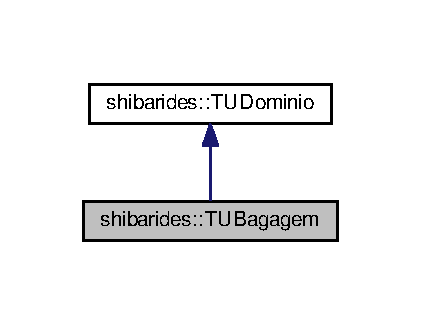
\includegraphics[width=202pt]{classshibarides_1_1TUBagagem__inherit__graph}
\end{center}
\end{figure}


Diagrama de colaboração para shibarides\+:\+:T\+U\+Bagagem\+:\nopagebreak
\begin{figure}[H]
\begin{center}
\leavevmode
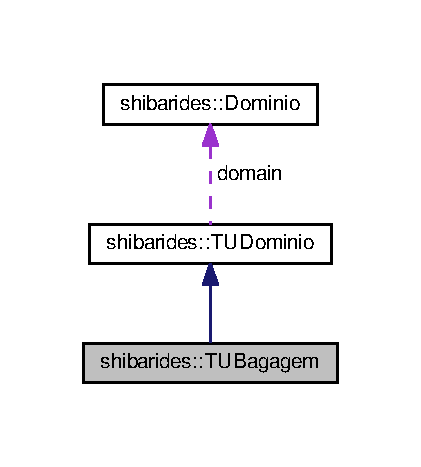
\includegraphics[width=202pt]{classshibarides_1_1TUBagagem__coll__graph}
\end{center}
\end{figure}
\subsection*{Outros membros herdados}


A documentação para esta classe foi gerada a partir dos seguintes arquivos\+:\begin{DoxyCompactItemize}
\item 
shibarides/Shiba\+Rides\+Domains\+U\+T.\+hpp\item 
shibarides/Shiba\+Rides\+Domains\+U\+T.\+cpp\end{DoxyCompactItemize}

\hypertarget{classshibarides_1_1TUCidade}{}\section{Referência da Classe shibarides\+:\+:T\+U\+Cidade}
\label{classshibarides_1_1TUCidade}\index{shibarides\+::\+T\+U\+Cidade@{shibarides\+::\+T\+U\+Cidade}}


Diagrama de Hierarquia para shibarides\+:\+:T\+U\+Cidade\+:\nopagebreak
\begin{figure}[H]
\begin{center}
\leavevmode
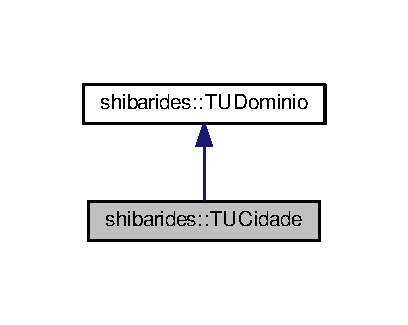
\includegraphics[width=196pt]{classshibarides_1_1TUCidade__inherit__graph}
\end{center}
\end{figure}


Diagrama de colaboração para shibarides\+:\+:T\+U\+Cidade\+:\nopagebreak
\begin{figure}[H]
\begin{center}
\leavevmode
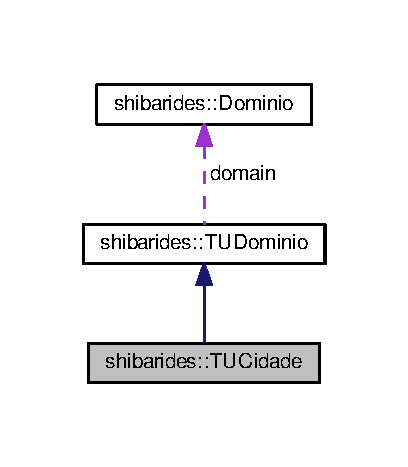
\includegraphics[width=196pt]{classshibarides_1_1TUCidade__coll__graph}
\end{center}
\end{figure}
\subsection*{Métodos Privados}
\begin{DoxyCompactItemize}
\item 
void {\bfseries gen\+Fail\+Values} ()\hypertarget{classshibarides_1_1TUCidade_ac9acc05f2f24dc5373db0e2865bc5ebe}{}\label{classshibarides_1_1TUCidade_ac9acc05f2f24dc5373db0e2865bc5ebe}

\item 
void {\bfseries gen\+Success\+Values} ()\hypertarget{classshibarides_1_1TUCidade_a794abad6cf007867b470091413cda5bd}{}\label{classshibarides_1_1TUCidade_a794abad6cf007867b470091413cda5bd}

\item 
void {\bfseries create\+Domain} ()\hypertarget{classshibarides_1_1TUCidade_a2d6b6611a3cb5245f22efba45c0d8e5c}{}\label{classshibarides_1_1TUCidade_a2d6b6611a3cb5245f22efba45c0d8e5c}

\end{DoxyCompactItemize}
\subsection*{Outros membros herdados}


A documentação para esta classe foi gerada a partir dos seguintes arquivos\+:\begin{DoxyCompactItemize}
\item 
shibarides/domains/Shiba\+Rides\+Domains\+U\+T.\+hpp\item 
shibarides/domains/Shiba\+Rides\+Domains\+U\+T.\+cpp\end{DoxyCompactItemize}

\hypertarget{classshibarides_1_1TUCodDeBanco}{}\section{Referência da Classe shibarides\+:\+:T\+U\+Cod\+De\+Banco}
\label{classshibarides_1_1TUCodDeBanco}\index{shibarides\+::\+T\+U\+Cod\+De\+Banco@{shibarides\+::\+T\+U\+Cod\+De\+Banco}}


Diagrama de Hierarquia para shibarides\+:\+:T\+U\+Cod\+De\+Banco\+:\nopagebreak
\begin{figure}[H]
\begin{center}
\leavevmode
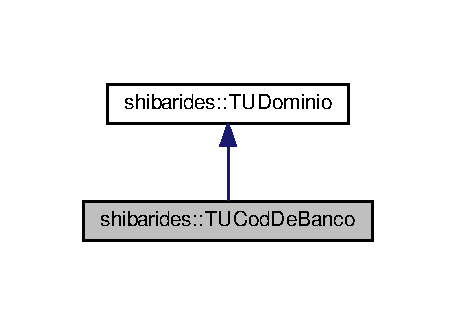
\includegraphics[width=219pt]{classshibarides_1_1TUCodDeBanco__inherit__graph}
\end{center}
\end{figure}


Diagrama de colaboração para shibarides\+:\+:T\+U\+Cod\+De\+Banco\+:\nopagebreak
\begin{figure}[H]
\begin{center}
\leavevmode
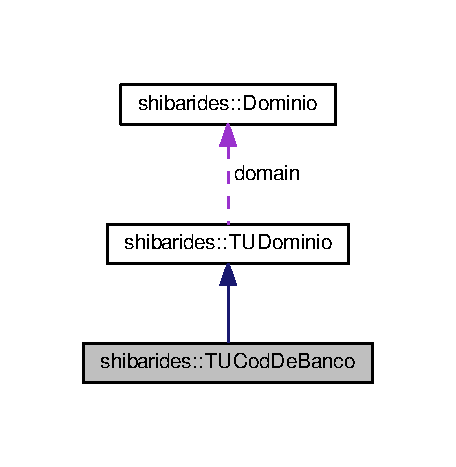
\includegraphics[width=219pt]{classshibarides_1_1TUCodDeBanco__coll__graph}
\end{center}
\end{figure}
\subsection*{Métodos Privados}
\begin{DoxyCompactItemize}
\item 
void {\bfseries gen\+Fail\+Values} ()\hypertarget{classshibarides_1_1TUCodDeBanco_a1be8519f0fd272ed30c8bf95129c0e73}{}\label{classshibarides_1_1TUCodDeBanco_a1be8519f0fd272ed30c8bf95129c0e73}

\item 
void {\bfseries gen\+Success\+Values} ()\hypertarget{classshibarides_1_1TUCodDeBanco_a5c3d2e95fe26d3a3620c277c0a97579b}{}\label{classshibarides_1_1TUCodDeBanco_a5c3d2e95fe26d3a3620c277c0a97579b}

\item 
void {\bfseries create\+Domain} ()\hypertarget{classshibarides_1_1TUCodDeBanco_a65d74f2fb107cb039c5abe74ebc0b1fc}{}\label{classshibarides_1_1TUCodDeBanco_a65d74f2fb107cb039c5abe74ebc0b1fc}

\end{DoxyCompactItemize}
\subsection*{Outros membros herdados}


A documentação para esta classe foi gerada a partir dos seguintes arquivos\+:\begin{DoxyCompactItemize}
\item 
shibarides/Shiba\+Rides\+Domains\+U\+T.\+hpp\item 
shibarides/Shiba\+Rides\+Domains\+U\+T.\+cpp\end{DoxyCompactItemize}

\hypertarget{classshibarides_1_1TUCodDeCarona}{}\section{Referência da Classe shibarides\+:\+:T\+U\+Cod\+De\+Carona}
\label{classshibarides_1_1TUCodDeCarona}\index{shibarides\+::\+T\+U\+Cod\+De\+Carona@{shibarides\+::\+T\+U\+Cod\+De\+Carona}}


Diagrama de Hierarquia para shibarides\+:\+:T\+U\+Cod\+De\+Carona\+:
% FIG 0


Diagrama de colaboração para shibarides\+:\+:T\+U\+Cod\+De\+Carona\+:
% FIG 1
\subsection*{Outros membros herdados}


A documentação para esta classe foi gerada a partir dos seguintes arquivos\+:\begin{DoxyCompactItemize}
\item 
shibarides/Shiba\+Rides\+Domains\+U\+T.\+hpp\item 
shibarides/Shiba\+Rides\+Domains\+U\+T.\+cpp\end{DoxyCompactItemize}

\hypertarget{classshibarides_1_1TUCodDeReserva}{}\section{Referência da Classe shibarides\+:\+:T\+U\+Cod\+De\+Reserva}
\label{classshibarides_1_1TUCodDeReserva}\index{shibarides\+::\+T\+U\+Cod\+De\+Reserva@{shibarides\+::\+T\+U\+Cod\+De\+Reserva}}


Diagrama de Hierarquia para shibarides\+:\+:T\+U\+Cod\+De\+Reserva\+:\nopagebreak
\begin{figure}[H]
\begin{center}
\leavevmode
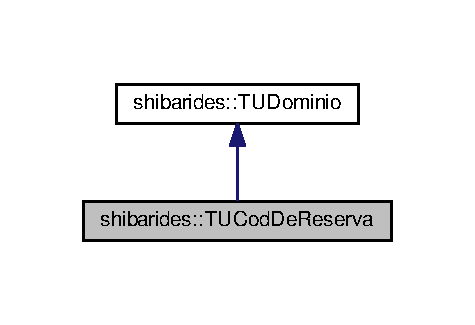
\includegraphics[width=228pt]{classshibarides_1_1TUCodDeReserva__inherit__graph}
\end{center}
\end{figure}


Diagrama de colaboração para shibarides\+:\+:T\+U\+Cod\+De\+Reserva\+:\nopagebreak
\begin{figure}[H]
\begin{center}
\leavevmode
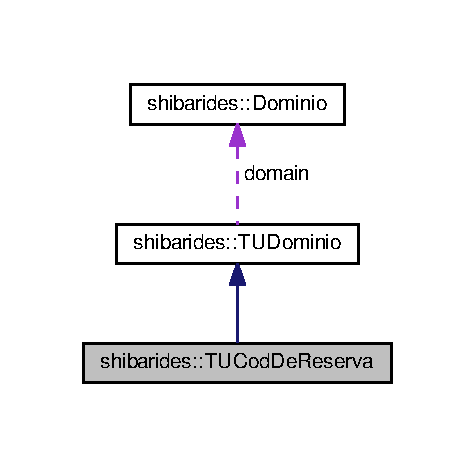
\includegraphics[width=228pt]{classshibarides_1_1TUCodDeReserva__coll__graph}
\end{center}
\end{figure}
\subsection*{Métodos Privados}
\begin{DoxyCompactItemize}
\item 
void {\bfseries gen\+Fail\+Values} ()\hypertarget{classshibarides_1_1TUCodDeReserva_a76b950ff521e9027410554ca9f57a75e}{}\label{classshibarides_1_1TUCodDeReserva_a76b950ff521e9027410554ca9f57a75e}

\item 
void {\bfseries gen\+Success\+Values} ()\hypertarget{classshibarides_1_1TUCodDeReserva_a2947a150417b195e862c34114291fe96}{}\label{classshibarides_1_1TUCodDeReserva_a2947a150417b195e862c34114291fe96}

\item 
void {\bfseries create\+Domain} ()\hypertarget{classshibarides_1_1TUCodDeReserva_af81ea709a8dbbebe6c66099698e4a191}{}\label{classshibarides_1_1TUCodDeReserva_af81ea709a8dbbebe6c66099698e4a191}

\end{DoxyCompactItemize}
\subsection*{Outros membros herdados}


A documentação para esta classe foi gerada a partir dos seguintes arquivos\+:\begin{DoxyCompactItemize}
\item 
shibarides/domains/Shiba\+Rides\+Domains\+U\+T.\+hpp\item 
shibarides/domains/Shiba\+Rides\+Domains\+U\+T.\+cpp\end{DoxyCompactItemize}

\hypertarget{classshibarides_1_1TUCPF}{}\section{Referência da Classe shibarides\+:\+:T\+U\+C\+PF}
\label{classshibarides_1_1TUCPF}\index{shibarides\+::\+T\+U\+C\+PF@{shibarides\+::\+T\+U\+C\+PF}}


Diagrama de Hierarquia para shibarides\+:\+:T\+U\+C\+PF\+:\nopagebreak
\begin{figure}[H]
\begin{center}
\leavevmode
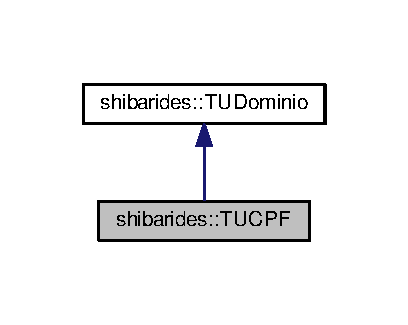
\includegraphics[width=196pt]{classshibarides_1_1TUCPF__inherit__graph}
\end{center}
\end{figure}


Diagrama de colaboração para shibarides\+:\+:T\+U\+C\+PF\+:\nopagebreak
\begin{figure}[H]
\begin{center}
\leavevmode
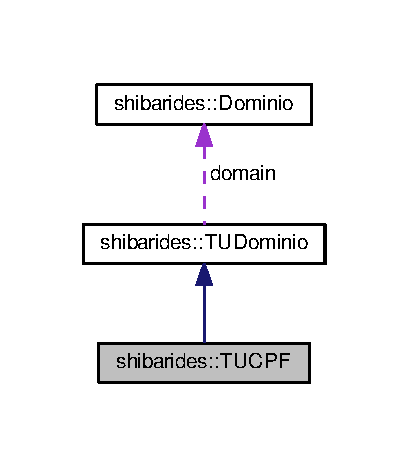
\includegraphics[width=196pt]{classshibarides_1_1TUCPF__coll__graph}
\end{center}
\end{figure}
\subsection*{Métodos Privados}
\begin{DoxyCompactItemize}
\item 
void {\bfseries gen\+Fail\+Values} ()\hypertarget{classshibarides_1_1TUCPF_a3cf74c1e8f7234dbe8735d82b79437f7}{}\label{classshibarides_1_1TUCPF_a3cf74c1e8f7234dbe8735d82b79437f7}

\item 
void {\bfseries gen\+Success\+Values} ()\hypertarget{classshibarides_1_1TUCPF_a1a8eb44e696ac200af8e6f5a35226ec0}{}\label{classshibarides_1_1TUCPF_a1a8eb44e696ac200af8e6f5a35226ec0}

\item 
void {\bfseries create\+Domain} ()\hypertarget{classshibarides_1_1TUCPF_a264f35c85b0b257ad62e913db84359f0}{}\label{classshibarides_1_1TUCPF_a264f35c85b0b257ad62e913db84359f0}

\end{DoxyCompactItemize}
\subsection*{Outros membros herdados}


A documentação para esta classe foi gerada a partir dos seguintes arquivos\+:\begin{DoxyCompactItemize}
\item 
shibarides/Shiba\+Rides\+Domains\+U\+T.\+hpp\item 
shibarides/Shiba\+Rides\+Domains\+U\+T.\+cpp\end{DoxyCompactItemize}

\hypertarget{classshibarides_1_1TUData}{}\section{Referência da Classe shibarides\+:\+:T\+U\+Data}
\label{classshibarides_1_1TUData}\index{shibarides\+::\+T\+U\+Data@{shibarides\+::\+T\+U\+Data}}


Diagrama de Hierarquia para shibarides\+:\+:T\+U\+Data\+:\nopagebreak
\begin{figure}[H]
\begin{center}
\leavevmode
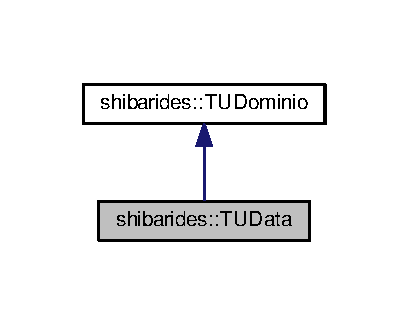
\includegraphics[width=196pt]{classshibarides_1_1TUData__inherit__graph}
\end{center}
\end{figure}


Diagrama de colaboração para shibarides\+:\+:T\+U\+Data\+:\nopagebreak
\begin{figure}[H]
\begin{center}
\leavevmode
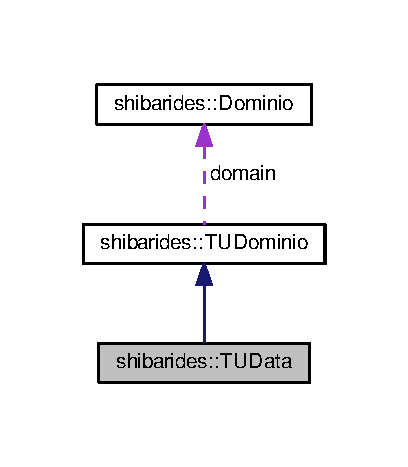
\includegraphics[width=196pt]{classshibarides_1_1TUData__coll__graph}
\end{center}
\end{figure}
\subsection*{Outros membros herdados}


A documentação para esta classe foi gerada a partir dos seguintes arquivos\+:\begin{DoxyCompactItemize}
\item 
shibarides/Shiba\+Rides\+Domains\+U\+T.\+hpp\item 
shibarides/Shiba\+Rides\+Domains\+U\+T.\+cpp\end{DoxyCompactItemize}

\hypertarget{classshibarides_1_1TUDominio}{}\section{Referência da Classe shibarides\+:\+:T\+U\+Dominio}
\label{classshibarides_1_1TUDominio}\index{shibarides\+::\+T\+U\+Dominio@{shibarides\+::\+T\+U\+Dominio}}


Diagrama de Hierarquia para shibarides\+:\+:T\+U\+Dominio\+:\nopagebreak
\begin{figure}[H]
\begin{center}
\leavevmode
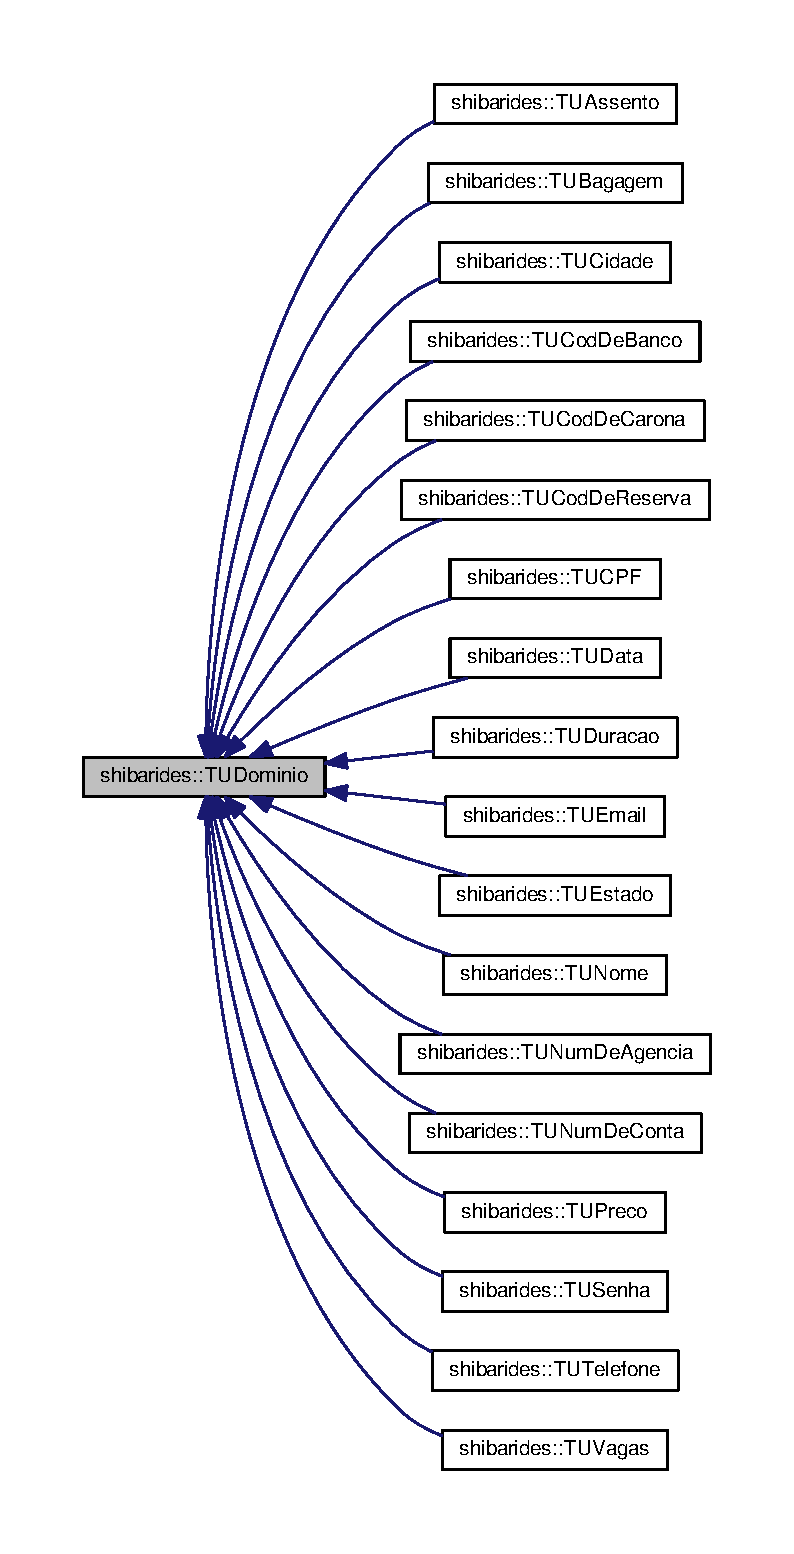
\includegraphics[height=550pt]{classshibarides_1_1TUDominio__inherit__graph}
\end{center}
\end{figure}


Diagrama de colaboração para shibarides\+:\+:T\+U\+Dominio\+:\nopagebreak
\begin{figure}[H]
\begin{center}
\leavevmode
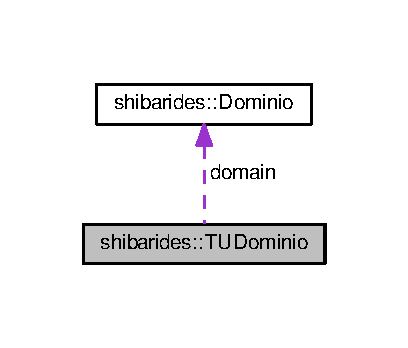
\includegraphics[width=196pt]{classshibarides_1_1TUDominio__coll__graph}
\end{center}
\end{figure}
\subsection*{Métodos Públicos}
\begin{DoxyCompactItemize}
\item 
int {\bfseries run} ()\hypertarget{classshibarides_1_1TUDominio_a3ed6438c91e763541b289e352d9d0d9d}{}\label{classshibarides_1_1TUDominio_a3ed6438c91e763541b289e352d9d0d9d}

\end{DoxyCompactItemize}
\subsection*{Atributos Estáticos Públicos}
\begin{DoxyCompactItemize}
\item 
static const int {\bfseries S\+U\+C\+C\+E\+SS} = 1\hypertarget{classshibarides_1_1TUDominio_aaed9469af819def9a9f2117e6c72d8b4}{}\label{classshibarides_1_1TUDominio_aaed9469af819def9a9f2117e6c72d8b4}

\item 
static const int {\bfseries F\+A\+IL} = 0\hypertarget{classshibarides_1_1TUDominio_a93c02894a2f820b9d2cefe501a2f06f5}{}\label{classshibarides_1_1TUDominio_a93c02894a2f820b9d2cefe501a2f06f5}

\end{DoxyCompactItemize}
\subsection*{Atributos Protegidos}
\begin{DoxyCompactItemize}
\item 
\hyperlink{classshibarides_1_1Dominio}{Dominio} $\ast$ {\bfseries domain}\hypertarget{classshibarides_1_1TUDominio_afbbf2e1d69e2a78b6d493521eb1a897f}{}\label{classshibarides_1_1TUDominio_afbbf2e1d69e2a78b6d493521eb1a897f}

\item 
int {\bfseries state}\hypertarget{classshibarides_1_1TUDominio_abfc3febebd253f31304997ea2715ac48}{}\label{classshibarides_1_1TUDominio_abfc3febebd253f31304997ea2715ac48}

\item 
std\+::vector$<$ std\+::string $>$ {\bfseries fail\+Values}\hypertarget{classshibarides_1_1TUDominio_ac1c9d98bd0e659ede32711ac693d6276}{}\label{classshibarides_1_1TUDominio_ac1c9d98bd0e659ede32711ac693d6276}

\item 
std\+::vector$<$ std\+::string $>$ {\bfseries success\+Values}\hypertarget{classshibarides_1_1TUDominio_a93df3635be9b1cd0726f5f1427a7b414}{}\label{classshibarides_1_1TUDominio_a93df3635be9b1cd0726f5f1427a7b414}

\end{DoxyCompactItemize}


A documentação para esta classe foi gerada a partir dos seguintes arquivos\+:\begin{DoxyCompactItemize}
\item 
shibarides/Shiba\+Rides\+Domains\+U\+T.\+hpp\item 
shibarides/Shiba\+Rides\+Domains\+U\+T.\+cpp\end{DoxyCompactItemize}

\hypertarget{classshibarides_1_1TUDuracao}{}\section{Referência da Classe shibarides\+:\+:T\+U\+Duracao}
\label{classshibarides_1_1TUDuracao}\index{shibarides\+::\+T\+U\+Duracao@{shibarides\+::\+T\+U\+Duracao}}


Diagrama de Hierarquia para shibarides\+:\+:T\+U\+Duracao\+:\nopagebreak
\begin{figure}[H]
\begin{center}
\leavevmode
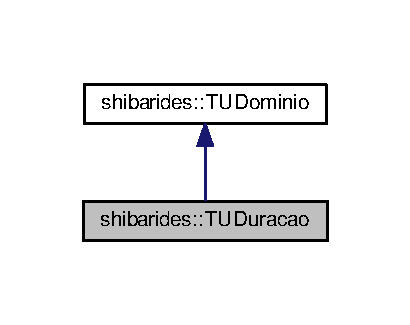
\includegraphics[width=197pt]{classshibarides_1_1TUDuracao__inherit__graph}
\end{center}
\end{figure}


Diagrama de colaboração para shibarides\+:\+:T\+U\+Duracao\+:\nopagebreak
\begin{figure}[H]
\begin{center}
\leavevmode
\includegraphics[width=197pt]{classshibarides_1_1TUDuracao__coll__graph}
\end{center}
\end{figure}
\subsection*{Outros membros herdados}


A documentação para esta classe foi gerada a partir dos seguintes arquivos\+:\begin{DoxyCompactItemize}
\item 
shibarides/Shiba\+Rides\+Domains\+U\+T.\+hpp\item 
shibarides/Shiba\+Rides\+Domains\+U\+T.\+cpp\end{DoxyCompactItemize}

\hypertarget{classshibarides_1_1TUEmail}{}\section{Referência da Classe shibarides\+:\+:T\+U\+Email}
\label{classshibarides_1_1TUEmail}\index{shibarides\+::\+T\+U\+Email@{shibarides\+::\+T\+U\+Email}}


Diagrama de Hierarquia para shibarides\+:\+:T\+U\+Email\+:
% FIG 0


Diagrama de colaboração para shibarides\+:\+:T\+U\+Email\+:
% FIG 1
\subsection*{Outros membros herdados}


A documentação para esta classe foi gerada a partir dos seguintes arquivos\+:\begin{DoxyCompactItemize}
\item 
shibarides/Shiba\+Rides\+Domains\+U\+T.\+hpp\item 
shibarides/Shiba\+Rides\+Domains\+U\+T.\+cpp\end{DoxyCompactItemize}

\hypertarget{classshibarides_1_1TUEstado}{}\section{Referência da Classe shibarides\+:\+:T\+U\+Estado}
\label{classshibarides_1_1TUEstado}\index{shibarides\+::\+T\+U\+Estado@{shibarides\+::\+T\+U\+Estado}}


Diagrama de Hierarquia para shibarides\+:\+:T\+U\+Estado\+:\nopagebreak
\begin{figure}[H]
\begin{center}
\leavevmode
\includegraphics[width=196pt]{classshibarides_1_1TUEstado__inherit__graph}
\end{center}
\end{figure}


Diagrama de colaboração para shibarides\+:\+:T\+U\+Estado\+:\nopagebreak
\begin{figure}[H]
\begin{center}
\leavevmode
\includegraphics[width=196pt]{classshibarides_1_1TUEstado__coll__graph}
\end{center}
\end{figure}
\subsection*{Métodos Privados}
\begin{DoxyCompactItemize}
\item 
void {\bfseries gen\+Fail\+Values} ()\hypertarget{classshibarides_1_1TUEstado_ab00d8cf1b69df380a241be507d84a044}{}\label{classshibarides_1_1TUEstado_ab00d8cf1b69df380a241be507d84a044}

\item 
void {\bfseries gen\+Success\+Values} ()\hypertarget{classshibarides_1_1TUEstado_a53162396ea238518f94d458285492970}{}\label{classshibarides_1_1TUEstado_a53162396ea238518f94d458285492970}

\item 
void {\bfseries create\+Domain} ()\hypertarget{classshibarides_1_1TUEstado_ab26d507b1cd22d6f47c3bf24d5a78c18}{}\label{classshibarides_1_1TUEstado_ab26d507b1cd22d6f47c3bf24d5a78c18}

\end{DoxyCompactItemize}
\subsection*{Outros membros herdados}


A documentação para esta classe foi gerada a partir dos seguintes arquivos\+:\begin{DoxyCompactItemize}
\item 
shibarides/domains/Shiba\+Rides\+Domains\+U\+T.\+hpp\item 
shibarides/domains/Shiba\+Rides\+Domains\+U\+T.\+cpp\end{DoxyCompactItemize}

\hypertarget{classshibarides_1_1TUNome}{}\section{Referência da Classe shibarides\+:\+:T\+U\+Nome}
\label{classshibarides_1_1TUNome}\index{shibarides\+::\+T\+U\+Nome@{shibarides\+::\+T\+U\+Nome}}


Diagrama de Hierarquia para shibarides\+:\+:T\+U\+Nome\+:
% FIG 0


Diagrama de colaboração para shibarides\+:\+:T\+U\+Nome\+:
% FIG 1
\subsection*{Outros membros herdados}


A documentação para esta classe foi gerada a partir dos seguintes arquivos\+:\begin{DoxyCompactItemize}
\item 
shibarides/Shiba\+Rides\+Domains\+U\+T.\+hpp\item 
shibarides/Shiba\+Rides\+Domains\+U\+T.\+cpp\end{DoxyCompactItemize}

\hypertarget{classshibarides_1_1TUNumDeAgencia}{}\section{Referência da Classe shibarides\+:\+:T\+U\+Num\+De\+Agencia}
\label{classshibarides_1_1TUNumDeAgencia}\index{shibarides\+::\+T\+U\+Num\+De\+Agencia@{shibarides\+::\+T\+U\+Num\+De\+Agencia}}


Diagrama de Hierarquia para shibarides\+:\+:T\+U\+Num\+De\+Agencia\+:
% FIG 0


Diagrama de colaboração para shibarides\+:\+:T\+U\+Num\+De\+Agencia\+:
% FIG 1
\subsection*{Outros membros herdados}


A documentação para esta classe foi gerada a partir dos seguintes arquivos\+:\begin{DoxyCompactItemize}
\item 
shibarides/Shiba\+Rides\+Domains\+U\+T.\+hpp\item 
shibarides/Shiba\+Rides\+Domains\+U\+T.\+cpp\end{DoxyCompactItemize}

\hypertarget{classshibarides_1_1TUNumDeConta}{}\section{Referência da Classe shibarides\+:\+:T\+U\+Num\+De\+Conta}
\label{classshibarides_1_1TUNumDeConta}\index{shibarides\+::\+T\+U\+Num\+De\+Conta@{shibarides\+::\+T\+U\+Num\+De\+Conta}}


Diagrama de Hierarquia para shibarides\+:\+:T\+U\+Num\+De\+Conta\+:\nopagebreak
\begin{figure}[H]
\begin{center}
\leavevmode
\includegraphics[width=220pt]{classshibarides_1_1TUNumDeConta__inherit__graph}
\end{center}
\end{figure}


Diagrama de colaboração para shibarides\+:\+:T\+U\+Num\+De\+Conta\+:\nopagebreak
\begin{figure}[H]
\begin{center}
\leavevmode
\includegraphics[width=220pt]{classshibarides_1_1TUNumDeConta__coll__graph}
\end{center}
\end{figure}
\subsection*{Métodos Privados}
\begin{DoxyCompactItemize}
\item 
void {\bfseries gen\+Fail\+Values} ()\hypertarget{classshibarides_1_1TUNumDeConta_af8cc65b26c3ed15ffe94c70cf46803a4}{}\label{classshibarides_1_1TUNumDeConta_af8cc65b26c3ed15ffe94c70cf46803a4}

\item 
void {\bfseries gen\+Success\+Values} ()\hypertarget{classshibarides_1_1TUNumDeConta_ac363d736ea593fe866657997e5f11a8a}{}\label{classshibarides_1_1TUNumDeConta_ac363d736ea593fe866657997e5f11a8a}

\item 
void {\bfseries create\+Domain} ()\hypertarget{classshibarides_1_1TUNumDeConta_ad1f293790ffc9a2c55ab3dbfa4422931}{}\label{classshibarides_1_1TUNumDeConta_ad1f293790ffc9a2c55ab3dbfa4422931}

\end{DoxyCompactItemize}
\subsection*{Outros membros herdados}


A documentação para esta classe foi gerada a partir dos seguintes arquivos\+:\begin{DoxyCompactItemize}
\item 
shibarides/domains/Shiba\+Rides\+Domains\+U\+T.\+hpp\item 
shibarides/domains/Shiba\+Rides\+Domains\+U\+T.\+cpp\end{DoxyCompactItemize}

\hypertarget{classshibarides_1_1TUPreco}{}\section{Referência da Classe shibarides\+:\+:T\+U\+Preco}
\label{classshibarides_1_1TUPreco}\index{shibarides\+::\+T\+U\+Preco@{shibarides\+::\+T\+U\+Preco}}


Diagrama de Hierarquia para shibarides\+:\+:T\+U\+Preco\+:\nopagebreak
\begin{figure}[H]
\begin{center}
\leavevmode
\includegraphics[width=196pt]{classshibarides_1_1TUPreco__inherit__graph}
\end{center}
\end{figure}


Diagrama de colaboração para shibarides\+:\+:T\+U\+Preco\+:\nopagebreak
\begin{figure}[H]
\begin{center}
\leavevmode
\includegraphics[width=196pt]{classshibarides_1_1TUPreco__coll__graph}
\end{center}
\end{figure}
\subsection*{Métodos Privados}
\begin{DoxyCompactItemize}
\item 
void {\bfseries gen\+Fail\+Values} ()\hypertarget{classshibarides_1_1TUPreco_a76bae658ac461a4a781a9967bb28b57a}{}\label{classshibarides_1_1TUPreco_a76bae658ac461a4a781a9967bb28b57a}

\item 
void {\bfseries gen\+Success\+Values} ()\hypertarget{classshibarides_1_1TUPreco_a6bf47d478080acf75e66df5128ff2a06}{}\label{classshibarides_1_1TUPreco_a6bf47d478080acf75e66df5128ff2a06}

\item 
void {\bfseries create\+Domain} ()\hypertarget{classshibarides_1_1TUPreco_a1b05bbbaad5fb145dd5373242f6b4cc8}{}\label{classshibarides_1_1TUPreco_a1b05bbbaad5fb145dd5373242f6b4cc8}

\end{DoxyCompactItemize}
\subsection*{Outros membros herdados}


A documentação para esta classe foi gerada a partir dos seguintes arquivos\+:\begin{DoxyCompactItemize}
\item 
shibarides/Shiba\+Rides\+Domains\+U\+T.\+hpp\item 
shibarides/Shiba\+Rides\+Domains\+U\+T.\+cpp\end{DoxyCompactItemize}

\hypertarget{classshibarides_1_1TUSenha}{}\section{Referência da Classe shibarides\+:\+:T\+U\+Senha}
\label{classshibarides_1_1TUSenha}\index{shibarides\+::\+T\+U\+Senha@{shibarides\+::\+T\+U\+Senha}}


Diagrama de Hierarquia para shibarides\+:\+:T\+U\+Senha\+:\nopagebreak
\begin{figure}[H]
\begin{center}
\leavevmode
\includegraphics[width=196pt]{classshibarides_1_1TUSenha__inherit__graph}
\end{center}
\end{figure}


Diagrama de colaboração para shibarides\+:\+:T\+U\+Senha\+:\nopagebreak
\begin{figure}[H]
\begin{center}
\leavevmode
\includegraphics[width=196pt]{classshibarides_1_1TUSenha__coll__graph}
\end{center}
\end{figure}
\subsection*{Métodos Privados}
\begin{DoxyCompactItemize}
\item 
void {\bfseries gen\+Fail\+Values} ()\hypertarget{classshibarides_1_1TUSenha_a36e77e3c35ed308d5b02ec1776ca1fc5}{}\label{classshibarides_1_1TUSenha_a36e77e3c35ed308d5b02ec1776ca1fc5}

\item 
void {\bfseries gen\+Success\+Values} ()\hypertarget{classshibarides_1_1TUSenha_a4a84474c545c06eaf95c6e90fd89e24a}{}\label{classshibarides_1_1TUSenha_a4a84474c545c06eaf95c6e90fd89e24a}

\item 
void {\bfseries create\+Domain} ()\hypertarget{classshibarides_1_1TUSenha_a31dfa215fd8c677220f9e3c79c9694fd}{}\label{classshibarides_1_1TUSenha_a31dfa215fd8c677220f9e3c79c9694fd}

\end{DoxyCompactItemize}
\subsection*{Outros membros herdados}


A documentação para esta classe foi gerada a partir dos seguintes arquivos\+:\begin{DoxyCompactItemize}
\item 
shibarides/Shiba\+Rides\+Domains\+U\+T.\+hpp\item 
shibarides/Shiba\+Rides\+Domains\+U\+T.\+cpp\end{DoxyCompactItemize}

\hypertarget{classshibarides_1_1TUTelefone}{}\section{Referência da Classe shibarides\+:\+:T\+U\+Telefone}
\label{classshibarides_1_1TUTelefone}\index{shibarides\+::\+T\+U\+Telefone@{shibarides\+::\+T\+U\+Telefone}}


Diagrama de Hierarquia para shibarides\+:\+:T\+U\+Telefone\+:\nopagebreak
\begin{figure}[H]
\begin{center}
\leavevmode
\includegraphics[width=198pt]{classshibarides_1_1TUTelefone__inherit__graph}
\end{center}
\end{figure}


Diagrama de colaboração para shibarides\+:\+:T\+U\+Telefone\+:\nopagebreak
\begin{figure}[H]
\begin{center}
\leavevmode
\includegraphics[width=198pt]{classshibarides_1_1TUTelefone__coll__graph}
\end{center}
\end{figure}
\subsection*{Métodos Privados}
\begin{DoxyCompactItemize}
\item 
void {\bfseries gen\+Fail\+Values} ()\hypertarget{classshibarides_1_1TUTelefone_ad5b7d969825572158769a8deeea35865}{}\label{classshibarides_1_1TUTelefone_ad5b7d969825572158769a8deeea35865}

\item 
void {\bfseries gen\+Success\+Values} ()\hypertarget{classshibarides_1_1TUTelefone_a4f099eb87da42f7f28b5ea4dd0d1edae}{}\label{classshibarides_1_1TUTelefone_a4f099eb87da42f7f28b5ea4dd0d1edae}

\item 
void {\bfseries create\+Domain} ()\hypertarget{classshibarides_1_1TUTelefone_a5d3f5bfcd7f13a7f381a41cc64e0a527}{}\label{classshibarides_1_1TUTelefone_a5d3f5bfcd7f13a7f381a41cc64e0a527}

\end{DoxyCompactItemize}
\subsection*{Outros membros herdados}


A documentação para esta classe foi gerada a partir dos seguintes arquivos\+:\begin{DoxyCompactItemize}
\item 
shibarides/domains/Shiba\+Rides\+Domains\+U\+T.\+hpp\item 
shibarides/domains/Shiba\+Rides\+Domains\+U\+T.\+cpp\end{DoxyCompactItemize}

\hypertarget{classshibarides_1_1TUVagas}{}\section{Referência da Classe shibarides\+:\+:T\+U\+Vagas}
\label{classshibarides_1_1TUVagas}\index{shibarides\+::\+T\+U\+Vagas@{shibarides\+::\+T\+U\+Vagas}}


Diagrama de Hierarquia para shibarides\+:\+:T\+U\+Vagas\+:\nopagebreak
\begin{figure}[H]
\begin{center}
\leavevmode
\includegraphics[width=196pt]{classshibarides_1_1TUVagas__inherit__graph}
\end{center}
\end{figure}


Diagrama de colaboração para shibarides\+:\+:T\+U\+Vagas\+:\nopagebreak
\begin{figure}[H]
\begin{center}
\leavevmode
\includegraphics[width=196pt]{classshibarides_1_1TUVagas__coll__graph}
\end{center}
\end{figure}
\subsection*{Métodos Privados}
\begin{DoxyCompactItemize}
\item 
void {\bfseries gen\+Fail\+Values} ()\hypertarget{classshibarides_1_1TUVagas_a18f9e781e747aceb5bc1d07cffa64d27}{}\label{classshibarides_1_1TUVagas_a18f9e781e747aceb5bc1d07cffa64d27}

\item 
void {\bfseries gen\+Success\+Values} ()\hypertarget{classshibarides_1_1TUVagas_a6c5d71f494a230732543277e1b6fd560}{}\label{classshibarides_1_1TUVagas_a6c5d71f494a230732543277e1b6fd560}

\item 
void {\bfseries create\+Domain} ()\hypertarget{classshibarides_1_1TUVagas_a3808426688f36963beab22b26a402270}{}\label{classshibarides_1_1TUVagas_a3808426688f36963beab22b26a402270}

\end{DoxyCompactItemize}
\subsection*{Outros membros herdados}


A documentação para esta classe foi gerada a partir dos seguintes arquivos\+:\begin{DoxyCompactItemize}
\item 
shibarides/domains/Shiba\+Rides\+Domains\+U\+T.\+hpp\item 
shibarides/domains/Shiba\+Rides\+Domains\+U\+T.\+cpp\end{DoxyCompactItemize}

\hypertarget{classshibarides_1_1Usuario}{}\section{Referência da Classe shibarides\+:\+:Usuario}
\label{classshibarides_1_1Usuario}\index{shibarides\+::\+Usuario@{shibarides\+::\+Usuario}}
\subsection*{Métodos Públicos}
\begin{DoxyCompactItemize}
\item 
void {\bfseries set\+Nome} (const \hyperlink{classshibarides_1_1Nome}{Nome} \&nome)\hypertarget{classshibarides_1_1Usuario_a605b73d80deba51209b16c15e7b93bd2}{}\label{classshibarides_1_1Usuario_a605b73d80deba51209b16c15e7b93bd2}

\item 
\hyperlink{classshibarides_1_1Nome}{Nome} {\bfseries get\+Nome} () const \hypertarget{classshibarides_1_1Usuario_ab85327f5d8942aca054561c6716e9d18}{}\label{classshibarides_1_1Usuario_ab85327f5d8942aca054561c6716e9d18}

\item 
void {\bfseries set\+Telefone} (const \hyperlink{classshibarides_1_1Telefone}{Telefone} \&telefone)\hypertarget{classshibarides_1_1Usuario_a2be45f53adbb82577dbe5821d767baed}{}\label{classshibarides_1_1Usuario_a2be45f53adbb82577dbe5821d767baed}

\item 
\hyperlink{classshibarides_1_1Telefone}{Telefone} {\bfseries get\+Telefone} () const \hypertarget{classshibarides_1_1Usuario_ad8658cd8fbe83ec38321849a88a48489}{}\label{classshibarides_1_1Usuario_ad8658cd8fbe83ec38321849a88a48489}

\item 
void {\bfseries set\+Email} (const \hyperlink{classshibarides_1_1Email}{Email} \&email)\hypertarget{classshibarides_1_1Usuario_a754f27880c0ce24072844655487554e5}{}\label{classshibarides_1_1Usuario_a754f27880c0ce24072844655487554e5}

\item 
\hyperlink{classshibarides_1_1Email}{Email} {\bfseries get\+Email} () const \hypertarget{classshibarides_1_1Usuario_ac78cb31456c8962980dcb5089bf60bee}{}\label{classshibarides_1_1Usuario_ac78cb31456c8962980dcb5089bf60bee}

\item 
void {\bfseries set\+Senha} (const \hyperlink{classshibarides_1_1Senha}{Senha} \&senha)\hypertarget{classshibarides_1_1Usuario_a089f1080a88d5170d210c69c77127b06}{}\label{classshibarides_1_1Usuario_a089f1080a88d5170d210c69c77127b06}

\item 
\hyperlink{classshibarides_1_1Senha}{Senha} {\bfseries get\+Senha} () const \hypertarget{classshibarides_1_1Usuario_a17d84322766046fc4457cce62b35daf9}{}\label{classshibarides_1_1Usuario_a17d84322766046fc4457cce62b35daf9}

\item 
void {\bfseries set\+C\+PF} (const \hyperlink{classshibarides_1_1CPF}{C\+PF} \&cpf)\hypertarget{classshibarides_1_1Usuario_ad22e4cf193a09a935b33ee6bc1b5102d}{}\label{classshibarides_1_1Usuario_ad22e4cf193a09a935b33ee6bc1b5102d}

\item 
\hyperlink{classshibarides_1_1CPF}{C\+PF} {\bfseries get\+C\+PF} () const \hypertarget{classshibarides_1_1Usuario_a9710f4d8e7c3ae151ee45f164a147b0c}{}\label{classshibarides_1_1Usuario_a9710f4d8e7c3ae151ee45f164a147b0c}

\end{DoxyCompactItemize}


A documentação para esta classe foi gerada a partir do seguinte arquivo\+:\begin{DoxyCompactItemize}
\item 
shibarides/Shiba\+Rides\+Entities.\+hpp\end{DoxyCompactItemize}

\hypertarget{classshibarides_1_1Vagas}{}\section{Referência da Classe shibarides\+:\+:Vagas}
\label{classshibarides_1_1Vagas}\index{shibarides\+::\+Vagas@{shibarides\+::\+Vagas}}


\hyperlink{classshibarides_1_1Dominio}{Dominio} responsável pela quantidade de vagas em uma carona.  




{\ttfamily \#include $<$Shiba\+Rides\+Domains.\+hpp$>$}



Diagrama de Hierarquia para shibarides\+:\+:Vagas\+:\nopagebreak
\begin{figure}[H]
\begin{center}
\leavevmode
\includegraphics[width=183pt]{classshibarides_1_1Vagas__inherit__graph}
\end{center}
\end{figure}


Diagrama de colaboração para shibarides\+:\+:Vagas\+:\nopagebreak
\begin{figure}[H]
\begin{center}
\leavevmode
\includegraphics[width=183pt]{classshibarides_1_1Vagas__coll__graph}
\end{center}
\end{figure}
\subsection*{Métodos Privados}
\begin{DoxyCompactItemize}
\item 
void \hyperlink{classshibarides_1_1Vagas_ae5f73c52819397524b0334d9e609d296}{validate} (std\+::string)  throw (std\+::invalid\+\_\+argument)
\begin{DoxyCompactList}\small\item\em Método que define as regras de validação para o dominio. \end{DoxyCompactList}\end{DoxyCompactItemize}
\subsection*{Outros membros herdados}


\subsection{Descrição Detalhada}
\hyperlink{classshibarides_1_1Dominio}{Dominio} responsável pela quantidade de vagas em uma carona. 

Representa as vagas disponíveis em uma carona dos usuários. Os valores devem ser de 0 a 4. 

\subsection{Métodos}
\index{shibarides\+::\+Vagas@{shibarides\+::\+Vagas}!validate@{validate}}
\index{validate@{validate}!shibarides\+::\+Vagas@{shibarides\+::\+Vagas}}
\subsubsection[{\texorpdfstring{validate(std\+::string)}{validate(std::string)}}]{\setlength{\rightskip}{0pt plus 5cm}void Vagas\+::validate (
\begin{DoxyParamCaption}
\item[{std\+::string}]{value}
\end{DoxyParamCaption}
) throw  std\+::invalid\+\_\+argument) \hspace{0.3cm}{\ttfamily [private]}, {\ttfamily [virtual]}}\hypertarget{classshibarides_1_1Vagas_ae5f73c52819397524b0334d9e609d296}{}\label{classshibarides_1_1Vagas_ae5f73c52819397524b0334d9e609d296}


Método que define as regras de validação para o dominio. 

O método validate implementa as regras de validação para o dominio. Os valores devem ser de 0 a 4.


\begin{DoxyParams}{Parâmetros}
{\em value} & Valor a ser validado \\
\hline
\end{DoxyParams}

\begin{DoxyExceptions}{Exceções}
{\em std\+::invalid\+\_\+argument} & Argumento invalido pelas regras do dominio \\
\hline
\end{DoxyExceptions}


Implementa \hyperlink{classshibarides_1_1Dominio_acc9445531455c072bbf708709aebbe55}{shibarides\+::\+Dominio}.



A documentação para esta classe foi gerada a partir dos seguintes arquivos\+:\begin{DoxyCompactItemize}
\item 
shibarides/Shiba\+Rides\+Domains.\+hpp\item 
shibarides/Shiba\+Rides\+Domains.\+cpp\end{DoxyCompactItemize}

%--- End generated contents ---

% Index
\backmatter
\newpage
\phantomsection
\clearemptydoublepage
\addcontentsline{toc}{chapter}{Índice}
\printindex

\end{document}
